%% 
%% Copyright 2019-2020 Elsevier Ltd
%% 
%% This file is part of the 'CAS Bundle'.
%% --------------------------------------
%% 
%% It may be distributed under the conditions of the LaTeX Project Public
%% License, either version 1.2 of this license or (at your option) any
%% later version.  The latest version of this license is in
%%    http://www.latex-project.org/lppl.txt
%% and version 1.2 or later is part of all distributions of LaTeX
%% version 1999/12/01 or later.
%% 
%% The list of all files belonging to the 'CAS Bundle' is
%% given in the file `manifest.txt'.
%% 
%% Template article for cas-dc documentclass for 
%% double column output.

%\documentclass[a4paper,fleqn,longmktitle]{cas-dc}
\documentclass[a4paper,fleqn]{cas-dc}

%\usepackage[numbers]{natbib}
%\usepackage[authoryear]{natbib}
% \usepackage[authoryear,longnamesfirst]{natbib}
\usepackage[numbers,sort&compress]{natbib}
\usepackage{algorithm}
\usepackage{algorithmic}
\usepackage{amsmath}
\usepackage{enumitem}
\usepackage{placeins}
\usepackage{capt-of}
% Uncomment and use as if needed
%\newtheorem{theorem}{Theorem}
%\newtheorem{lemma}[theorem]{Lemma}
%\newdefinition{rmk}{Remark}
%\newproof{pf}{Proof}
%\newproof{pot}{Proof of Theorem \ref{thm}}

\begin{document}
\let\WriteBookmarks\relax
\setkeys{Gin}{interpolate=true}
\setcounter{topnumber}{3}
\setcounter{dbltopnumber}{3}
\setcounter{totalnumber}{5}
\renewcommand{\topfraction}{0.95}
\renewcommand{\dbltopfraction}{0.95}
\renewcommand{\textfraction}{0.05}
\renewcommand{\floatpagefraction}{0.75}
\renewcommand{\dblfloatpagefraction}{0.75}
\setlength{\textfloatsep}{8pt plus 2pt minus 2pt}
\setlength{\dbltextfloatsep}{8pt plus 2pt minus 2pt}
\setlength{\floatsep}{6pt plus 2pt minus 2pt}
\setlength{\dblfloatsep}{6pt plus 2pt minus 2pt}
\setlength{\intextsep}{6pt plus 2pt minus 2pt}
\setlength{\abovecaptionskip}{4pt}
\setlength{\belowcaptionskip}{0pt}
\setlist[itemize]{topsep=2pt,itemsep=2pt,parsep=0pt,partopsep=0pt}

% Short title
\shorttitle{BRACE: Boundary-Reliability Knowledge Alignment}

% Short author
\shortauthors{Y. Hu et~al.}

% Main title of the paper
\title [mode = title]{BRACE: A Boundary-Reliability Knowledge Alignment Framework for Semi-Supervised Ultrasound Segmentation
}                      
\hypersetup{
  pdftitle={BRACE: A Boundary-Reliability Knowledge Alignment Framework for Semi-Supervised Ultrasound Segmentation}
}
% Title footnote mark
% eg: \tnotemark[1]
% \tnotemark[1,2]

% Title footnote 1.
% eg: \tnotetext[1]{Title footnote text}
% \tnotetext[<tnote number>]{<tnote text>} 
% \tnotetext[1]{This document is the results of the research
%    project funded by the National Science Foundation.}

% \tnotetext[2]{The second title footnote which is a longer text matter
%    to fill through the whole text width and overflow into
%    another line in the footnotes area of the first page.}


% First author
%
% Options: Use if required
\author[1]{Yan Hu}[
% type=editor,
      % style=chinese,
      % auid=000,
      % bioid=1,
      % prefix=Sir,
      % orcid=0000-0000-0000-0000,
      % facebook=<facebook id>,
      % twitter=<twitter id>,
      % linkedin=<linkedin id>,
      % gplus=<gplus id>
      ]
\credit{Conceptualization of this study, Methodology, Software, Data curation, Writing - Original draft preparation, Writing - Review \& editing}
\ead{yh657@exeter.ac.uk}

% URL of the first author
% \ead[url]{www.cvr.cc, cvr@sayahna.org}

%  Credit authorship
% 
% \credit{}
\author[1]{Ming Yin}[
% type=editor,
      % style=chinese,
      % auid=000,
      % bioid=1,
      % prefix=Sir,
      % orcid=0000-0000-0000-0000,
      % facebook=<facebook id>,
      % twitter=<twitter id>,
      % linkedin=<linkedin id>,
      % gplus=<gplus id>
      ]
\credit{Conceptualization of this study, Methodology, Software, Writing - Review \& editing}
\ead{my417@exeter.ac.uk}

% URL of the first author
% \ead[url]{www.cvr.cc, cvr@sayahna.org}

%  Credit authorship
\author[1]{Mohammed M. Abdelsamea}[
% type=editor,
      % style=chinese,
      % auid=000,
      % bioid=1,
      % prefix=Sir,
      % orcid=0000-0000-0000-0000,
      % facebook=<facebook id>,
      % twitter=<twitter id>,
      % linkedin=<linkedin id>,
      % gplus=<gplus id>
      ]  
\credit{Writing - Review \& editing}
\ead{M.Abdelsamea@exeter.ac.uk}

% URL of the first author
% \ead[url]{www.cvr.cc, cvr@sayahna.org}

%  Credit authorship

\author[1]{Sareh Rowlands}[
% type=editor,
      % style=chinese,
      % auid=000,
      % bioid=1,
      % prefix=Sir,
      % orcid=0000-0000-0000-0000,
      % facebook=<facebook id>,
      % twitter=<twitter id>,
      % linkedin=<linkedin id>,
      % gplus=<gplus id>
      ]  
\credit{Writing - Review \& editing}
\ead{s.rowlands@exeter.ac.uk}

% URL of the first author
% \ead[url]{www.cvr.cc, cvr@sayahna.org}

%  Credit authorship
\author[1]{Lei Zhang}[
% type=editor,
      % style=chinese,
      % auid=000,
      % bioid=1,
      % prefix=Sir,
      % orcid=0000-0000-0000-0000,
      % facebook=<facebook id>,
      % twitter=<twitter id>,
      % linkedin=<linkedin id>,
      % gplus=<gplus id>
      ]
\credit{Writing - Review \& editing}
\ead{L.Zhang6@exeter.ac.uk}

% URL of the first author
% \ead[url]{www.cvr.cc, cvr@sayahna.org}

%  Credit authorship

\author[1]{Lu Liu}[
% type=editor,
      % style=chinese,
      % auid=000,
      % bioid=1,
      % prefix=Sir,
      % orcid=0000-0000-0000-0000,
      % facebook=<facebook id>,
      % twitter=<twitter id>,
      % linkedin=<linkedin id>,
      % gplus=<gplus id>
      ]  
\credit{Writing - Review \& editing}
\ead{L.Liu3@exeter.ac.uk}

% URL of the first author
% \ead[url]{www.cvr.cc, cvr@sayahna.org}

%  Credit authorship

\author[1]{Xujiong Ye}[
% type=editor,
      % style=chinese,
      % auid=000,
      % bioid=1,
      % prefix=Sir,
      % orcid=0000-0000-0000-0000,
      % facebook=<facebook id>,
      % twitter=<twitter id>,
      % linkedin=<linkedin id>,
      % gplus=<gplus id>
      ]  

      % % Email id of the first author
\credit{Writing - Review \& editing}
\ead{X.Ye2@exeter.ac.uk }

% URL of the first author
% \ead[url]{www.cvr.cc, cvr@sayahna.org}

%  Credit authorship

\author[1]{Zeyu Fu}[
% type=editor,
%                         auid=000,bioid=1,
%                         prefix=Sir,
%                         role=Researcher,
%                         orcid=0000-0001-7511-2910]
]
% Corresponding author indication
\cormark[1]

% Footnote of the first author
% \fnmark[1]

% % Email id of the first author
\credit{Conceptualization of this study, Methodology, Software, Writing - Review \& editing}
\ead{z.fu@exeter.ac.uk}

% URL of the first author
% \ead[url]{www.cvr.cc, cvr@sayahna.org}

%  Credit authorship
% \credit{Conceptualization of this study, Methodology, Software}

% Address/affiliation
\affiliation[1]{organization={Department of Computer Science, University of Exeter},
    % addressline={Radarweg 29}, 
    city={Exeter},
    % citysep={}, % Uncomment if no comma needed between city and postcode
    % postcode={1043 NX}, 
    % state={},
    country={UK}}

% Second author
% \author[2,4]{Han Theh Thanh}[style=chinese]

% Third author
% \author[2,3]{CV Rajagopal}[%
%    role=Co-ordinator,
%    suffix=Jr,
%    ]
% \fnmark[2]
% \ead{cvr3@sayahna.org}
% \ead[URL]{www.sayahna.org}



% Address/affiliation
% \affiliation[2]{organization={Sayahna Foundation},
%     % addressline={}, 
%     city={Jagathy},
%     % citysep={}, % Uncomment if no comma needed between city and postcode
%     postcode={695014}, 
%     state={Trivandrum},
%     country={India}}

% Fourth author
% \author%
% [1,3]
% {Rishi T.}
% \cormark[2]
% \fnmark[1,3]
% \ead{rishi@stmdocs.in}
% \ead[URL]{www.stmdocs.in}

% \affiliation[3]{organization={STM Document Engineering Pvt Ltd.},
%     addressline={Mepukada}, 
%     city={Malayinkil},
%     % citysep={}, % Uncomment if no comma needed between city and postcode
%     postcode={695571}, 
%     state={Trivandrum},
%     country={India}}

% Corresponding author text
\cortext[cor1]{Corresponding author}
% \cortext[cor2]{Principal corresponding author}

% Footnote text
% \fntext[fn1]{This is the first author footnote. but is common to third
  % author as well.}
% \fntext[fn2]{Another author footnote, this is a very long footnote and
  % it should be a really long footnote. But this footnote is not yet
  % sufficiently long enough to make two lines of footnote text.}

% For a title note without a number/mark
% \nonumnote{Emails:
%   }

% Here goes the abstract
\begin{abstract}
\textbf{Background and Objective:} Semi-supervised ultrasound segmentation is hindered by scarce pixel annotations and pseudo-label errors that often appear as boundary drift, fragmented contours, or implausible structures. We address this problem from a knowledge-based perspective by explicitly representing anatomical boundary knowledge and reliability knowledge during pseudo-label transfer.

\textbf{Methods:} We propose BRACE, a \textit{Boundary-Reliability Knowledge Alignment} framework built on a teacher--student dual-decoder network. BRACE combines three modules: \textit{Feature-Boundary Wasserstein Alignment} (FBWA), which aligns feature--boundary representations of labeled and unlabeled samples with a gradient-penalized Wasserstein critic; \textit{Structure-Oriented Residual Perturbation} (SORP), which constructs an auxiliary structure-sensitive view; and \textit{Reliability-Calibrated Co-teaching} (RCT), which weights pseudo-label supervision by entropy-derived reliability while applying boundary calibration and decoder agreement.

\textbf{Results:} Under the reference evaluation protocols of Shape Prior for BUSI/TN3K and BiPCC for PSFHS/HC18, BRACE achieves competitive segmentation performance across lesion and fetal-ultrasound tasks. Representative protocol-aligned results include 85.89\% DSC on TN3K with 1/2 labels, 83.66\% DSC on TN3K with 1/8 labels, 82.32\%/92.61\% DSC for PS/FH on PSFHS with 20\% labels, and 96.88\%/97.01\% DSC on HC18 with 10\%/20\% labels. Component analyses further support the contribution of reliability-calibrated boundary knowledge transfer.

\textbf{Conclusions:} BRACE provides a knowledge-guided mechanism for aligning structural boundary information with reliability-aware pseudo-label learning. The results support boundary-reliability alignment as a useful direction for low-annotation ultrasound segmentation, while broader multi-seed validation can further strengthen the statistical characterization of the framework.

\end{abstract}

% Use if graphical abstract is present
% \begin{graphicalabstract}
% \includegraphics{figs/grabs.pdf}
% \end{graphicalabstract}

% Keywords
% Each keyword is seperated by \sep
\begin{keywords}
Knowledge-based systems \sep Ultrasound segmentation \sep Semi-supervised learning \sep Boundary-reliability knowledge alignment \sep Medical decision support
\end{keywords}


\maketitle
\hypersetup{
  pdfauthor={Yan Hu, Ming Yin, Mohammed M. Abdelsamea, Sareh Rowlands, Lei Zhang, Lu Liu, Xujiong Ye, Zeyu Fu},
  pdfkeywords={Knowledge-based systems, Ultrasound segmentation, Semi-supervised learning, Boundary-reliability knowledge alignment, Medical decision support}
}

\section{Introduction}

Ultrasound (US) imaging is widely used in clinical practice for its safety, portability, and real-time acquisition. Accurate US segmentation supports lesion characterization, treatment planning, and longitudinal monitoring~\cite{b1,b4}, but obtaining pixel-level annotations is costly and expert-dependent~\cite{b4,b28}. Semi-supervised learning (SSL) addresses this by leveraging abundant unlabeled data alongside limited labeled samples~\cite{b5,b38,b33}. Representative SSL strategies include consistency regularization~\cite{b19,b32}, pseudo-labeling~\cite{b13,b38}, and teacher--student frameworks~\cite{b19}, which have shown success in medical imaging. Nevertheless, in ultrasound, low contrast, speckle noise, and high structural variability (Fig.~\ref{fig:lesion_variants}) make pseudo-supervision particularly prone to error; the core question is whether existing SSL mechanisms can transfer reliable \emph{anatomical knowledge} rather than merely enforce pixel-level agreement.

\noindent\begin{minipage}{\linewidth}
    \centering
    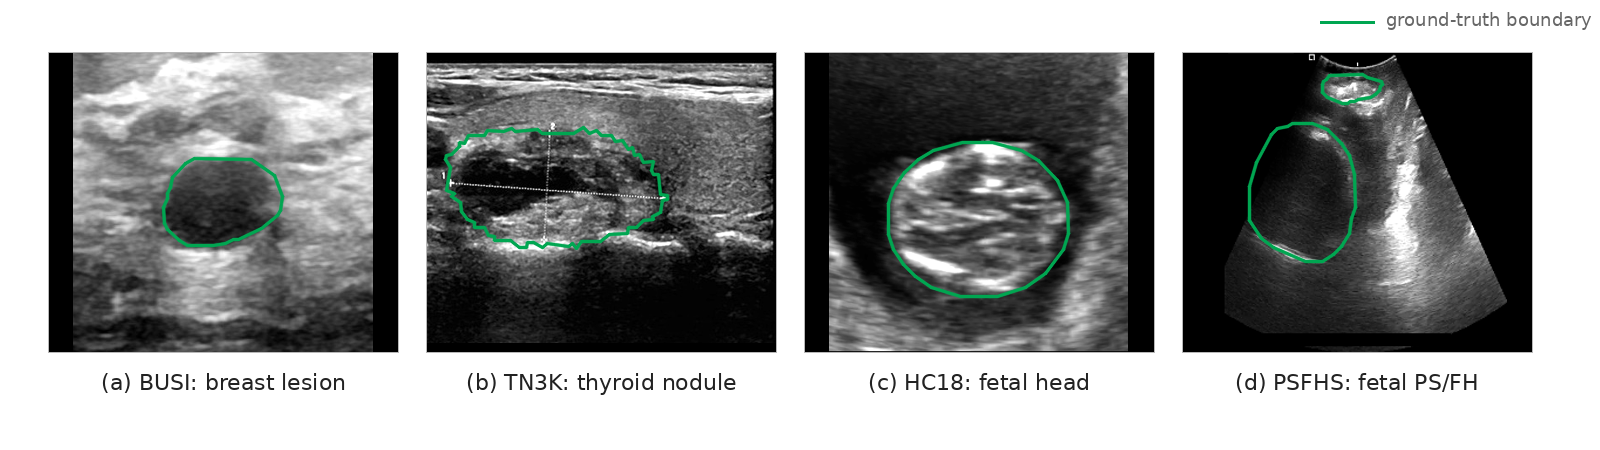
\includegraphics[width=1\linewidth]{intro_lesion_variants.png}
    \captionof{figure}{Challenging properties of ultrasound segmentation: (a) diverse lesion shapes and textures; (b) severe boundary ambiguity; (c) pseudo-label artifacts with irregular structures; (d) speckle noise interference. These cases highlight the need for knowledge-level boundary representation and reliability-aware pseudo-label transfer.}
    \label{fig:lesion_variants}
\end{minipage}
\par\smallskip

A central limitation of standard SSL segmentation is that pseudo-label errors are effectively treated as \emph{independent pixel-wise noise}; consistency losses then encourage agreement per pixel without guaranteeing global anatomical coherence. In ultrasound, however, errors are often \emph{structurally correlated}---e.g., contour drift or fragmented boundaries---so that pixel-level consistency can preserve local appearance while \emph{failing to maintain global shape fidelity}~\cite{b20,b38} (Fig.~\ref{fig:lesion_variants}(c)). In knowledge-based terms, teacher predictions contain two inseparable sources of information: \emph{structural boundary knowledge}, which describes how anatomical regions should be organized, and \emph{reliability knowledge}, which indicates where pseudo-supervision can be trusted. Existing objectives usually transfer only the hard or soft mask and therefore discard much of this boundary-reliability knowledge. Recent work has added shape or edge cues via hand-crafted regularizers~\cite{b56,b60,b61,b62,b63} or global shape discriminators~\cite{b2}; the former often rely on fixed geometric constraints that do not generalize across heterogeneous US data, while the latter typically operate on the full mask without decoder-level or boundary-level knowledge alignment, leaving structural uncertainty and decoder-induced distortion under-addressed.

In this work we establish BRACE, a boundary-reliability knowledge alignment framework for semi-supervised ultrasound segmentation. The method is motivated by two observations: pseudo-labels should be aligned with anatomical boundaries at the representation level, and unreliable unlabeled supervision should be adaptively down-weighted rather than treated uniformly. BRACE therefore integrates three mechanisms: (1) \emph{Feature-Boundary Wasserstein Alignment} (FBWA), which aligns deep features and boundary maps as structural knowledge; (2) \emph{Structure-Oriented Residual Perturbation} (SORP), which creates a prediction-guided auxiliary knowledge view by residual feature perturbation; and (3) \emph{Reliability-Calibrated Co-teaching} (RCT), which uses entropy-derived reliability together with boundary calibration and main--auxiliary decoder agreement to transfer pseudo-label knowledge. Together, these mechanisms acquire, align, and transfer boundary-reliability knowledge under scarce labeled data (Fig.~\ref{fig:detailed}).

Experiments on four public US datasets (BUSI~\cite{b1}, TN3K~\cite{b4}, PSFHS~\cite{b53}, HC18~\cite{b54}) under labeled ratios 1/8--1/2 demonstrate that BRACE is a competitive knowledge-guided SSL framework. To support reproducible interpretation, we explicitly follow the Shape Prior protocol for BUSI/TN3K and the BiPCC protocol for PSFHS/HC18, and report component ablations and sensitivity analyses under the same low-label settings.

The main contributions are:

\begin{itemize}
    \item We formulate semi-supervised ultrasound segmentation as a \emph{boundary-reliability knowledge transfer} problem, where the model must represent anatomical boundary knowledge and decide which pseudo-label knowledge is reliable enough to transfer.
    \item We propose BRACE, a knowledge-guided teacher--student framework that jointly aligns structural boundary knowledge and reliability knowledge through FBWA, SORP, and RCT.
    \item We design FBWA to align deep features with boundary representations through a Wasserstein-style critic, SORP to generate a perturbation-based auxiliary knowledge view, and RCT to perform reliability-calibrated pseudo-label co-teaching.
    \item We evaluate BRACE on BUSI, TN3K, PSFHS, and HC18 with region and boundary metrics, and provide ablations, sensitivity analysis, and limitation analysis to characterize its behavior under the reference protocols.
\end{itemize}

\section{Related Work}

We organize related work from a knowledge-transfer perspective. Existing SSL methods mainly transfer pixel-level pseudo-label knowledge; shape-prior methods inject mask-level structural knowledge; boundary-aware methods introduce local edge knowledge; and uncertainty-aware methods estimate reliability but often do not couple it with structural knowledge. BRACE is positioned at the intersection of these lines: it represents boundary knowledge, estimates reliability knowledge, and aligns both during teacher--student pseudo-label transfer.

\begin{figure*}[!t]
  \centering
  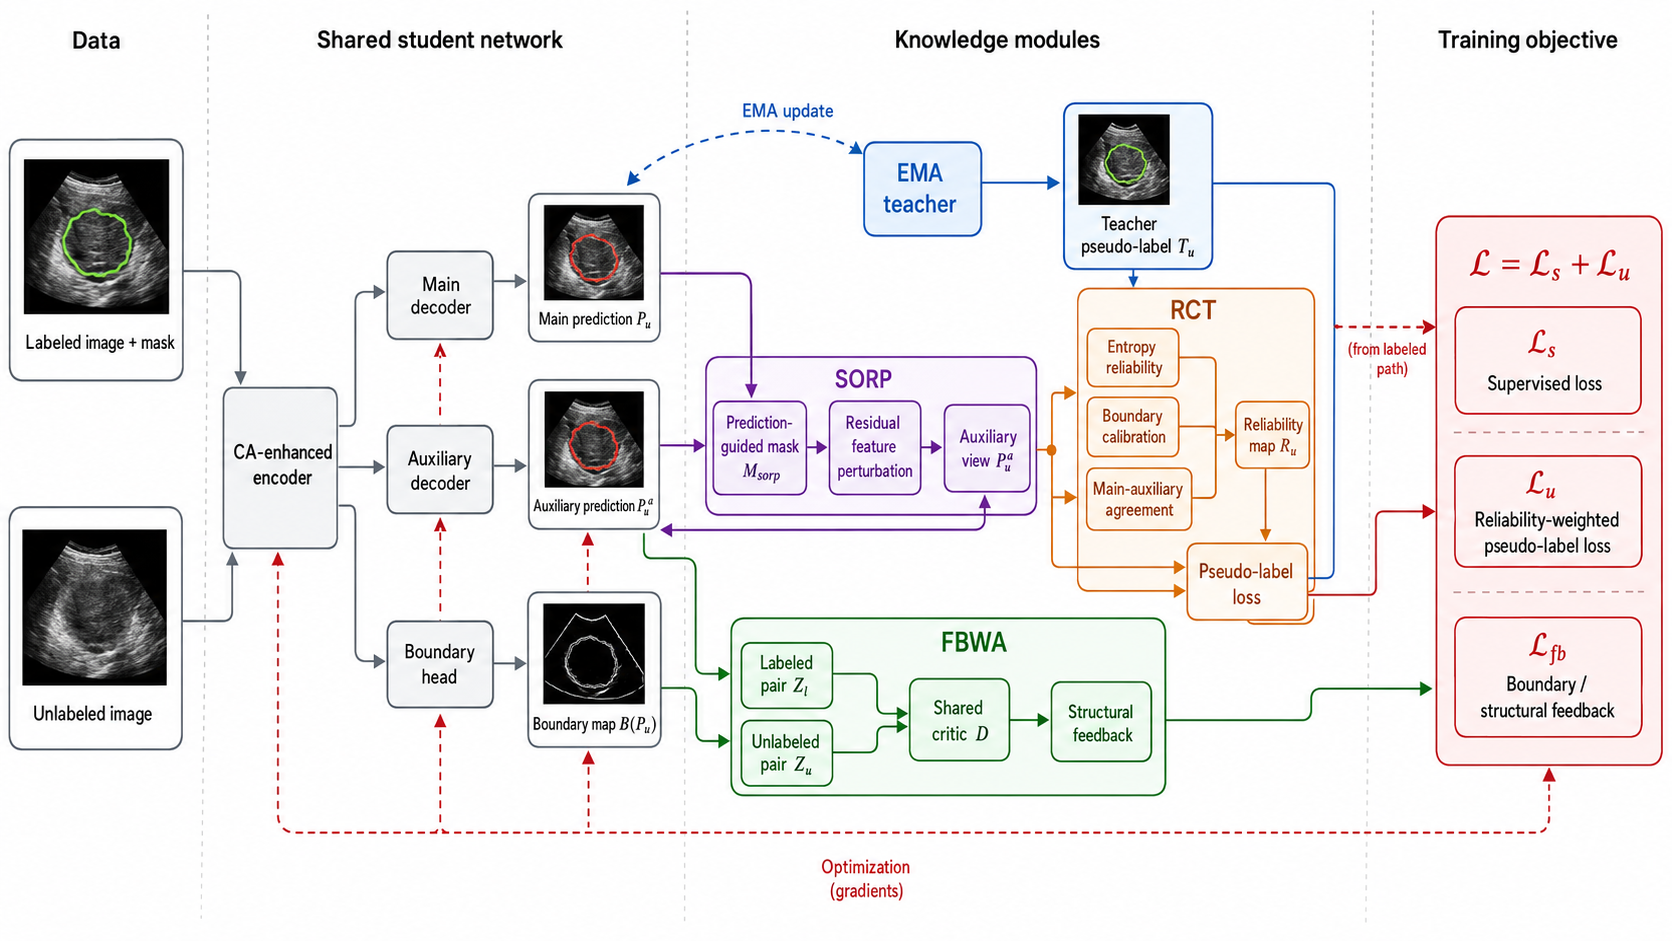
\includegraphics[width=0.98\linewidth]{user_overall_framework_notitle.png}
  \caption{Overview of BRACE as boundary-reliability knowledge alignment. FBWA represents structural boundary knowledge with feature--boundary pairs, SORP generates a perturbation-based auxiliary knowledge view, and RCT uses entropy-derived reliability, boundary calibration, and main--auxiliary co-teaching to transfer pseudo-label knowledge.}
  \label{fig:detailed}
\end{figure*}

\subsection{Pseudo-label Knowledge Transfer in SSL}

Consistency regularization encourages agreement between model outputs under different perturbations or views~\cite{b19,b18,b35}. The $\Pi$-model, Temporal Ensembling~\cite{b19}, Mean Teacher~\cite{b19}, and adaptations such as FixMatch~\cite{b18} and UA-MT~\cite{b21} rely on \emph{pixel-level} or prediction-level agreement. Pseudo-labeling (Pseudo-Label~\cite{b13}, CPS~\cite{b15}) transfers model predictions as targets, usually with confidence thresholding or augmentation consistency. These methods can be interpreted as transferring output knowledge from a teacher or peer model to the student. However, in ultrasound, pseudo-label errors are often \emph{structurally correlated} (e.g., contour drift or fragmented boundaries), so transferring only pixel-wise knowledge can propagate boundary drift across decoding stages rather than correct it. \textbf{Knowledge gap:} pixel-level pseudo-label transfer does not explicitly encode anatomical boundary knowledge or the reliability of different structural regions.

\subsection{Structural Priors and Boundary Knowledge}

To improve anatomical plausibility, several works add \emph{global} shape or mask-level constraints. Shape-Prior~\cite{b2} uses an adversarial discriminator on the full binary mask in a twin-decoder setup, penalizing implausible global shapes and improving structural coherence. MGCC~\cite{b65} uses a latent diffusion model to generate synthetic ultrasound and enforces multi-level cross-context consistency. Boundary-guided consistency~\cite{b60,b61}, shape-aligned regularization~\cite{b62,b63}, and structure-aware designs such as RA-BUSSeg~\cite{b56} introduce edge or shape terms via auxiliary losses or hand-crafted regularizers. These methods inject useful structural knowledge, but most operate either on the final mask or on local gradients. \textbf{Knowledge gap:} mask-level or edge-level priors do not fully align deep semantic features with boundary evidence, and they rarely provide a mechanism to decide when structural pseudo-knowledge should be trusted.

\subsection{Reliability Modeling for Pseudo-label Learning}

Reliability and uncertainty modeling are widely used to reduce confirmation bias in semi-supervised medical segmentation. Confidence thresholds, entropy weighting, teacher--student uncertainty, and multi-view agreement can suppress unreliable pseudo-labels before they dominate training. Nevertheless, reliability is frequently modeled as a scalar or pixel-wise weight attached to the pseudo-label target, while the structural source of the error is not explicitly represented. For boundary-ambiguous ultrasound, this separation is suboptimal: a pseudo-label region may be confident inside homogeneous areas but unreliable near semantic boundaries. \textbf{Knowledge gap:} reliability knowledge and boundary knowledge should be modeled jointly rather than as independent losses. BRACE addresses this gap by aligning feature--boundary knowledge through FBWA, constructing a perturbation-based auxiliary knowledge view through SORP, and transferring pseudo-label knowledge through RCT only in reliable regions.


\section{Method}

When pseudo-label errors are structurally correlated, pixel-wise consistency objectives may propagate boundary drift across decoding stages instead of correcting it. BRACE therefore treats semi-supervised ultrasound segmentation as boundary-reliability knowledge alignment: structural boundary knowledge should be represented in the feature space, and reliability knowledge should determine how pseudo-label knowledge is transferred. The following subsections formalize the setting and then detail how FBWA, SORP, and RCT implement this knowledge-based training process.

\subsection{Setting and Notation}

We consider semi-supervised segmentation with a labeled set $\mathcal{D}_l = \{(x_i, y_i)\}_{i=1}^{N_l}$ and an unlabeled set $\mathcal{D}_u = \{x_j\}_{j=1}^{N_u}$, where $N_u \gg N_l$. The goal is to learn a segmentation model $f_\theta: \mathcal{X} \rightarrow \mathcal{Y}$ (parameters $\theta$) that generalizes well with limited labels. We denote the supervised loss by $\mathcal{L}_s$ (on labeled data) and the unsupervised loss by $\mathcal{L}_u$, which aggregates structural alignment and consistency terms applied to unlabeled data. Pseudo-labels for unlabeled samples are generated by a teacher network (see below); no separate confidence threshold is applied beyond binarization of the teacher output when used as targets for the discriminator and consistency losses.

\subsection{Overall Framework}

BRACE adopts a teacher--student framework~\cite{b19} with a dual-decoder design (Fig.~\ref{fig:detailed}). The teacher and student share the same backbone: a CA-enhanced encoder~\cite{b7} and two decoders (main and auxiliary). The teacher parameters are an exponential moving average (EMA) of the student~\cite{b19}; its predictions on unlabeled images provide pseudo-label knowledge. The student is trained with supervised labels, reliability-calibrated pseudo-labels, FBWA structural feedback, and main--auxiliary co-teaching.

\paragraph{Revisiting the learning objective under structurally correlated errors.} The standard unsupervised objective encourages agreement between student and teacher predictions (e.g., pixel-wise or region-wise). When pseudo-label errors are \emph{structurally correlated} rather than independent across pixels, this objective can be satisfied by matching local appearance while leaving global shape or boundary errors uncorrected. To close this gap, the unsupervised term should (i) represent semantic boundary knowledge, (ii) create a perturbation-aware auxiliary knowledge view, and (iii) transfer pseudo-label knowledge according to reliability. FBWA, SORP, and RCT implement these requirements, respectively.

\subsection{Boundary-Reliability Knowledge Representation}

BRACE represents the information used in semi-supervised training as three coupled knowledge sources. First, \emph{structural boundary knowledge} $\mathcal{K}_b$ is encoded by feature--boundary pairs $Z=(A(F),\mathcal{B}(P))$, where $F$ is a deep semantic feature, $A(\cdot)$ is a feature adapter, $P$ is a segmentation mask or prediction, and $\mathcal{B}(\cdot)$ extracts boundary evidence. Second, \emph{reliability knowledge} $\mathcal{K}_r$ is represented by an entropy-derived reliability map. Boundary calibration and main--auxiliary decoder agreement are modeled as complementary training terms rather than being folded into $R_u$. Third, \emph{auxiliary perturbation knowledge} $\mathcal{K}_a$ is obtained from the SORP view, which tests whether the segmentation remains stable under prediction-guided residual perturbations. The goal of BRACE is not to impose a fixed anatomical template, but to align these knowledge sources so that unlabeled supervision is both anatomically plausible and reliability-aware.

The training objective is $\mathcal{L}=\mathcal{L}_s+\mathcal{L}_u$. For labeled data, $\mathcal{L}_s$ supervises the main decoder, auxiliary decoder, and boundary head. For unlabeled data, $\mathcal{L}_u$ aggregates reliability-weighted pseudo-label learning, main--auxiliary cross-teaching, and FBWA structural feedback. The architecture and data flow are detailed in Fig.~\ref{fig:detailed} and Sections~\ref{sec:fbwa}--\ref{sec:rcc}.

\subsection{Coordinate Attention-enhanced Encoder}
To improve spatial sensitivity and localization in low-contrast ultrasound images, we adopt the Coordinate Attention (CA) mechanism~\cite{b7} as an existing technique to enhance encoder features extracted from a ResNet34 backbone. Conventional CNN backbones such as ResNet34 are effective in extracting semantic representations but often compromise spatial precision due to repeated pooling and stride operations, which can be detrimental when segmenting lesions with ambiguous or diffuse boundaries. The integration of CA modules within the encoder structure is shown in the detailed architecture (Fig.~\ref{fig:detailed}).

\subsubsection{Multi-Scale Feature Enhancement}
Specifically, the encoder first extracts multi-scale features $\{e_1, e_2, e_3, e_4, e_5\}$ from the input image. These encoder outputs are then processed by CA modules to produce attention-enhanced features $\{f_1^{\text{att}}, f_2^{\text{att}}, f_3^{\text{att}}, f_4^{\text{att}}, s_5\}$, where $s_5$ denotes the CA-enhanced deepest feature.

\subsubsection{Directional Dependency Modeling}

Unlike conventional channel attention that aggregates global features without positional awareness, CA decomposes spatial attention into height and width directions, thereby encoding both positional and contextual information. Given a feature map $F \in \mathbb{R}^{C \times H \times W}$, where $C$ is the number of channels, $H$ is the height, and $W$ is the width, CA first performs directional pooling to capture long-range dependencies along each axis:
\begin{equation}
f^h(c, x) = \frac{1}{H} \sum_{y=1}^{H} F(c, y, x), \quad 
f^w(c, y) = \frac{1}{W} \sum_{x=1}^{W} F(c, y, x),
\end{equation}
where $f^h \in \mathbb{R}^{C \times W}$ and $f^w \in \mathbb{R}^{C \times H}$ are the aggregated features along the height and width dimensions, respectively. The resulting one-dimensional descriptors $f^h$ and $f^w$ are fused and transformed through lightweight convolutions to produce axis-specific attention maps, which are then applied to recalibrate the original feature map:
\begin{equation}
F' = F \cdot \sigma(f^h) \cdot \sigma(f^w),
\end{equation}
where $\sigma(\cdot)$ denotes the sigmoid activation function.

CA modules are embedded after each residual block:
\begin{equation}
F_i^{CA} = \text{CA}(F_i), \quad \text{for } i \in \{1, 2, 3, 4, 5\},
\end{equation}
which enables multi-scale enhancement of boundary-relevant and structurally significant features. The refined features are transmitted to the decoder via skip connections, ensuring that spatial information is preserved throughout the network.

As supported by the component study (Table~\ref{tab:ablation_full}), the CA-enhanced encoder contributes to more stable foreground segmentation under low-label settings. Moreover, CA introduces only marginal computational overhead, maintaining real-time feasibility. Both the ResNet34 backbone and CA modules are jointly optimized in an end-to-end manner.

\subsection{Dual-Decoder Architecture}

The CA-enhanced encoder features are fed into two parallel decoders: a main decoder and an auxiliary decoder. The main decoder produces the primary segmentation output $P$, whereas the auxiliary decoder receives SORP-perturbed encoder features and provides an alternative structural view. Rather than treating the auxiliary output as a stand-alone regularizer, BRACE couples the two decoders through reliability-calibrated pseudo-label learning and cross-teaching, as detailed in Section~\ref{sec:rcc}.



\subsection{Feature-Boundary Wasserstein Alignment (FBWA)}
\label{sec:fbwa}

FBWA implements structural boundary knowledge alignment. Unlike global shape discriminators that operate only on binary masks~\cite{b2}, FBWA evaluates whether deep features and boundary evidence form anatomically plausible joint representations. This design is important for ultrasound images, where local intensity cues can be ambiguous but boundary-feature compatibility remains informative.

\begin{figure*}[!t]
  \centering
  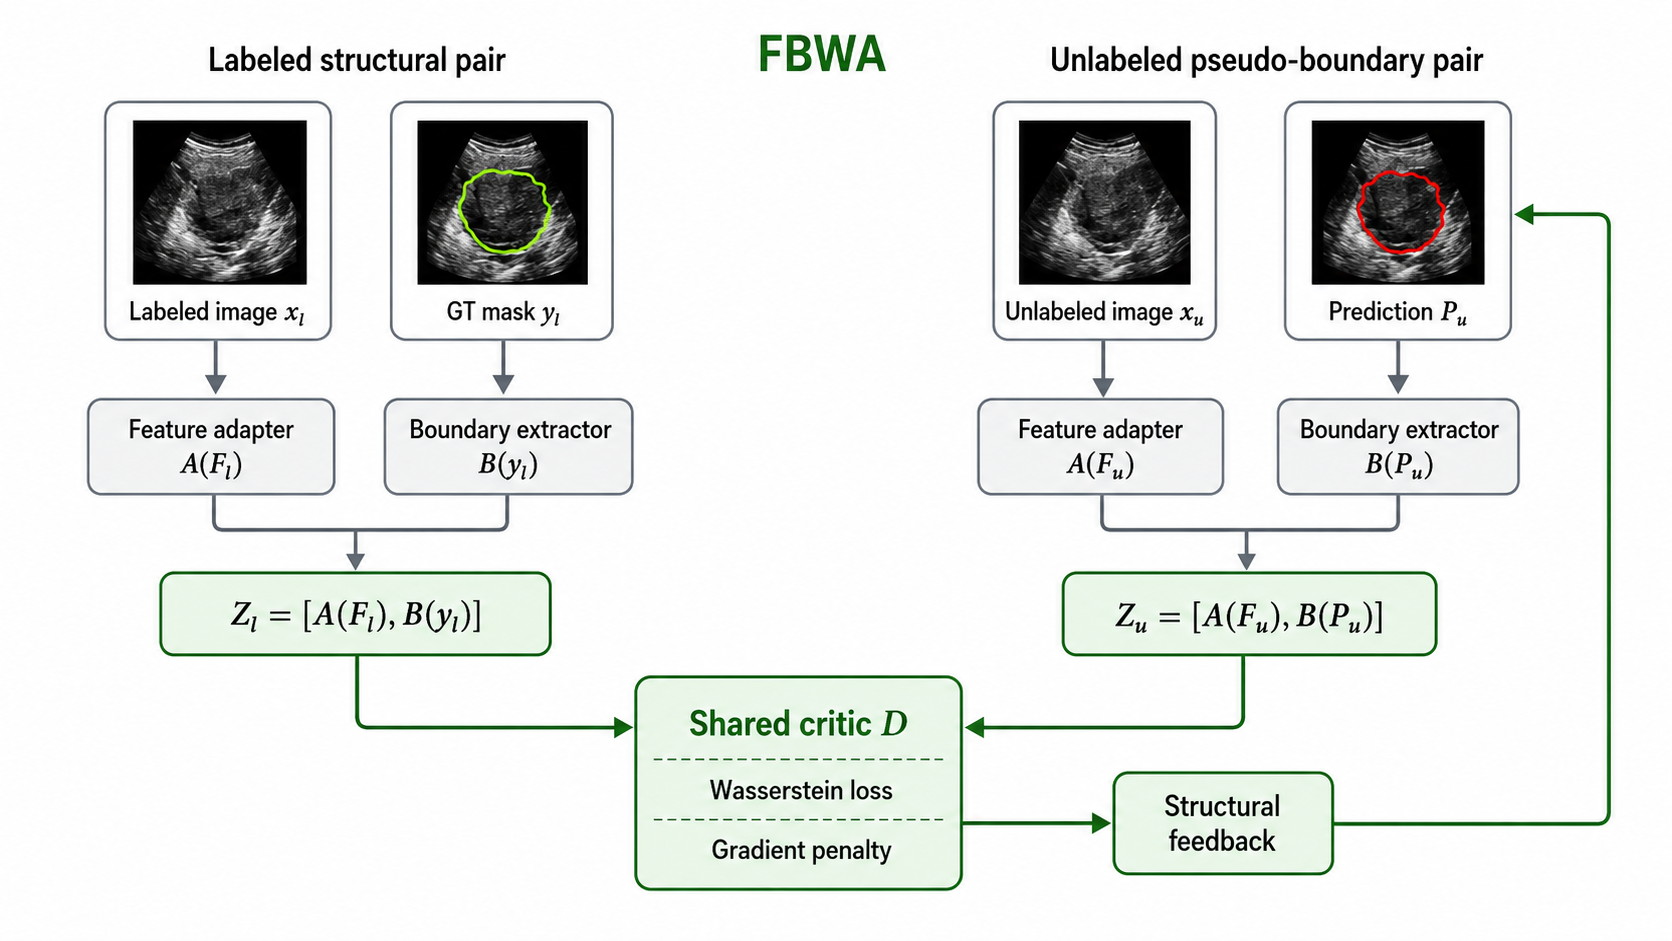
\includegraphics[width=0.98\linewidth]{user_fbwa_module_notitle.png}
  \caption{Feature-Boundary Wasserstein Alignment (FBWA). The critic receives concatenated feature--boundary pairs as structural boundary knowledge and provides feedback through a Wasserstein-style objective regularized by gradient penalty. This encourages pseudo-boundaries to be compatible with deep semantic representations.}
  \label{fig:scd}
\end{figure*}

Given a labeled image $x_l$ and an unlabeled image $x_u$, the encoder extracts deep features $F_l$ and $F_u$. We compute boundary maps with a Sobel operator $\mathcal{G}(\cdot)$ from the ground-truth mask $y_l$ and the unlabeled prediction $P_u$:
\begin{equation}
\mathcal{B}(P)=\sqrt{(G_x*P)^2+(G_y*P)^2},
\end{equation}
where $G_x$ and $G_y$ are horizontal and vertical Sobel kernels. A lightweight adapter $A(\cdot)$ maps the encoder feature to the critic input space, and the joint feature-boundary representations are defined as
\begin{equation}
Z_l=\operatorname{Concat}(A(F_l),\mathcal{B}(y_l)),\quad
Z_u=\operatorname{Concat}(A(F_u),\mathcal{B}(P_u)).
\end{equation}
For PSFHS, PS/FH boundaries are represented as two structural channels; for binary datasets, the second channel is zero-padded to keep a unified critic interface.

We train a critic $D$ with a Wasserstein-style objective regularized by WGAN-GP:
\begin{equation}
\mathcal{L}_{D}=\mathbb{E}[D(Z_u)]-\mathbb{E}[D(Z_l)]
+\lambda_{\rm gp}\mathbb{E}_{\hat{Z}}\big(\|\nabla_{\hat{Z}}D(\hat{Z})\|_2-1\big)^2 .
\end{equation}
The default reported code path uses the gradient penalty without applying a bounded critic clamp. The segmentation network receives the generator-side structural feedback
\begin{equation}
\mathcal{L}_{\rm FBWA}=-\mathbb{E}[D(Z_u)].
\end{equation}
Intuitively, FBWA does not force a fixed geometric prior; instead, it penalizes feature--boundary knowledge configurations that are unlikely under labeled anatomical structures.

\subsection{Structure-Oriented Residual Perturbation (SORP)}
\label{sec:sorp}

SORP creates a perturbation-aware auxiliary knowledge view without introducing a separate hand-crafted structural loss. Given the deepest feature $F$ and the current prediction $P$, we first derive a foreground confidence mask and sample a guided cutout region inside the predicted structure. The perturbed feature is formed by residual blending:
\begin{equation}
\tilde{F}=\rho F+(1-\rho)\big(F\odot M_{\rm sorp}(P)\big),
\end{equation}
where $M_{\rm sorp}(P)$ denotes the prediction-guided soft cutout mask and $\rho$ controls residual preservation. The auxiliary decoder receives $\tilde{F}$ and produces $P_u^{a}$. This residual design avoids overly destructive perturbations for small or uncertain structures while still exposing the model to structure-sensitive feature variations that serve as auxiliary knowledge.

SORP differs from conventional output-level perturbation consistency. Its role is to construct an informative auxiliary view; the consistency between the main output $P_u$ and auxiliary output $P_u^{a}$ is learned through RCT, so unreliable regions can be down-weighted instead of being forced to match uniformly. Fig.~\ref{fig:sorp_rct} illustrates how the SORP auxiliary view is coupled with RCT reliability estimation.

\subsection{Reliability-Calibrated Co-teaching (RCT)}
\label{sec:rcc}

RCT calibrates how pseudo-label knowledge is transferred from the EMA teacher to the student. Let $T_u$ be the teacher prediction for an unlabeled image. We define an entropy-based reliability map
\begin{equation}
R_u=\exp\big(-H(T_u)/\tau\big),
\end{equation}
where $H(\cdot)$ is pixel-wise entropy and $\tau$ is a temperature. Ambiguous pixels therefore contribute less to pseudo-supervision, reducing confirmation bias in low-contrast or boundary-ambiguous regions.

The main and auxiliary decoders are trained with reliability-weighted pseudo-label losses:
\begin{equation}
\mathcal{L}_{\rm PL}= \ell(P_u,T_u;R_u)+\lambda_{\rm pa} \ell(P_u^{a},T_u;R_u),
\end{equation}
where $\ell(\cdot)$ denotes a reliability-weighted BCE-Dice loss. For PSFHS, the implementation supports a class-aware weighted Dice option to handle PS/FH imbalance; a merged-foreground objective is also evaluated in the component analysis. In all cases, the boundary head is calibrated by the teacher-induced boundary map:
\begin{equation}
\mathcal{L}_{\rm BC}= \ell_b(B_u,\mathcal{B}(T_u);R_u).
\end{equation}
Finally, the two decoders exchange soft targets through reliability-weighted cross-teaching:
\begin{equation}
\mathcal{L}_{\rm CT}= \ell(P_u,\operatorname{sg}(P_u^{a});R_u)+\lambda_{\rm pa} \ell(P_u^{a},\operatorname{sg}(P_u);R_u),
\end{equation}
where $\operatorname{sg}(\cdot)$ stops gradients. RCT therefore transfers auxiliary SORP knowledge only where the prediction is reliable, rather than enforcing uniform agreement.


\begin{figure*}[!t]
  \centering
  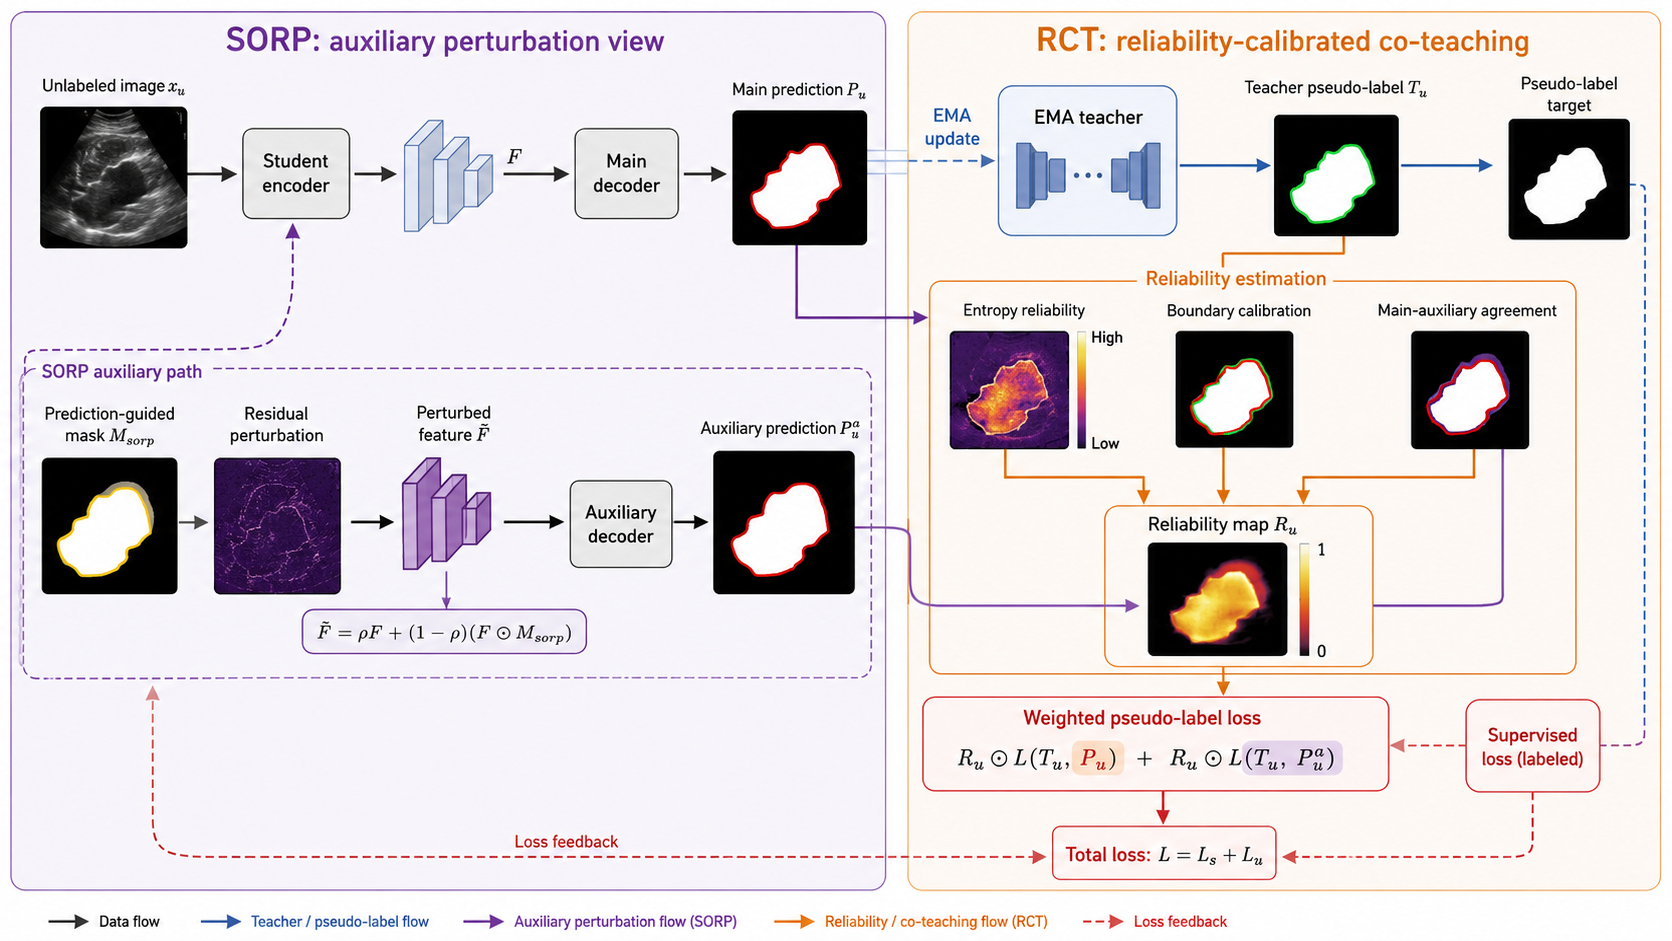
\includegraphics[width=0.98\linewidth]{sorp_rct_module.png}
  \caption{Structure-Oriented Residual Perturbation (SORP) and Reliability-Calibrated Co-teaching (RCT). SORP constructs an auxiliary prediction view through prediction-guided residual feature perturbation, while RCT uses entropy-derived reliability to weight pseudo-label supervision, together with boundary calibration and main--auxiliary co-teaching. Dashed arrows indicate auxiliary-view or loss-contribution paths.}
  \label{fig:sorp_rct}
\end{figure*}

\subsection{Learning Objectives}

The overall objective is
\begin{equation}
\mathcal{L}_{\rm total}=\mathcal{L}_{s}+\mathcal{L}_{u}.
\end{equation}
For labeled data, the supervised term combines main-decoder supervision, auxiliary-decoder supervision, and boundary supervision:
\begin{equation}
\mathcal{L}_{s}=\mathcal{L}_{\rm main}+\lambda_{\rm aux}\mathcal{L}_{\rm aux}+\lambda_b\mathcal{L}_{\rm bd}.
\end{equation}
For unlabeled data, the unsupervised term is
\begin{equation}
\mathcal{L}_{u}=\mathcal{L}_{\rm PL}+\lambda_{\rm bc}\mathcal{L}_{\rm BC}+\lambda_{\rm ct}\mathcal{L}_{\rm CT}+r_{\rm fbwa}(t)\lambda_{\rm adv}\mathcal{L}_{\rm FBWA},
\end{equation}
where $r_{\rm fbwa}(t)$ is a ramp-up coefficient for the FBWA critic. A Gaussian schedule $\lambda(t)=\alpha\exp[-\beta(1-t/T)^2]$ is used to gradually activate pseudo-label and cross-teaching terms. The current default implementation uses Adam optimization, EMA momentum 0.999, $\lambda_{\rm aux}=0.5$ for labeled auxiliary supervision, $\lambda_{\rm pa}=0.3$ for auxiliary pseudo-supervision, $\lambda_b=0.2$ for labeled boundary supervision, $\lambda_{\rm bc}=0.1$ for boundary calibration, $\lambda_{\rm ct}=0.3$ for main--auxiliary cross-teaching, and $\lambda_{\rm adv}=0.05$ for FBWA feedback. SORP supplies an auxiliary view in the current code path rather than an independent standalone SORP loss.

\subsection{Training Algorithm}

Algorithm~\ref{alg:training} summarizes the BRACE training procedure. The key difference from standard teacher--student SSL is that pseudo-label knowledge transfer is filtered by reliability, while the auxiliary SORP view and FBWA critic provide boundary-reliability knowledge alignment.

\begin{algorithm}[t]
\caption{BRACE Boundary-Reliability Knowledge Alignment Procedure}
\label{alg:training}
\begin{algorithmic}[1]
\REQUIRE Labeled dataset $\mathcal{D}_l$, unlabeled dataset $\mathcal{D}_u$, student network $f_\theta$, EMA teacher $f_{\theta'}$, FBWA critic $D$.
\ENSURE Trained segmentation model $f_\theta$.
\STATE Initialize $f_\theta$ and set $f_{\theta'} \leftarrow f_\theta$; initialize or load the FBWA critic.
\FOR{epoch $=1$ to $E$}
    \FOR{each labeled batch $(x_l,y_l)$ and unlabeled batch $x_u$}
        \STATE Predict labeled masks, auxiliary masks, and boundaries with the student.
        \STATE Compute $\mathcal{L}_s$ from main, auxiliary, and boundary supervision.
        \STATE Generate teacher pseudo-label $T_u=f_{\theta'}(x_u)$ and reliability map $R_u=\exp(-H(T_u)/\tau)$.
        \STATE Apply SORP to obtain a perturbed auxiliary view and compute $\mathcal{L}_{\rm PL}$, $\mathcal{L}_{\rm BC}$, and $\mathcal{L}_{\rm CT}$.
        \STATE Build feature-boundary pairs $Z_l$ and $Z_u$; update the FBWA critic with the Wasserstein-style loss and gradient penalty.
        \STATE Update the student with $\mathcal{L}_{\rm total}$.
        \STATE Update the teacher by EMA: $\theta' \leftarrow \mu\theta' + (1-\mu)\theta$.
    \ENDFOR
\ENDFOR
\end{algorithmic}
\end{algorithm}

\section{Experiments}

\subsection{Datasets and Labeled/Unlabeled Splits}

We evaluate on four public ultrasound segmentation datasets: \textbf{BUSI}~\cite{b1}, \textbf{TN3K}~\cite{b4}, \textbf{PSFHS}~\cite{b53}, and \textbf{HC18}~\cite{b54}. The BUSI/TN3K protocols follow the Shape Prior setting~\cite{b2}, and the PSFHS/HC18 protocols follow the fetal ultrasound setting used by BiPCC~\cite{b51}. We use these public reference partitions to maximize comparability with prior semi-supervised ultrasound segmentation studies.

\textbf{BUSI}~\cite{b1}: the BUSI dataset contains 780 breast ultrasound images. Following the Shape Prior protocol, we use the 647 benign and malignant images, with 576 images for training and 71 images for protocol evaluation. The labeled subsets contain 72, 144, and 288 images for the $1/8$, $1/4$, and $1/2$ protocols, respectively, and the remaining training images are treated as unlabeled.

\textbf{TN3K}~\cite{b4}: TN3K contains 3,493 thyroid nodule ultrasound images. Following the Shape Prior protocol, 2,578 images are used for training, 301 for validation, and 614 for testing. We use 322, 644, and 1,289 labeled training images for the $1/8$, $1/4$, and $1/2$ labeled protocols, respectively, and use the remaining training images as unlabeled data.

\textbf{PSFHS}~\cite{b53}: the Pubic Symphysis--Fetal Head Segmentation and Angle of Progression task is to segment the pubic symphysis (PS) and fetal head (FH). The BiPCC-aligned image-level protocol used in our experiments contains 4,000 two-dimensional intrapartum ultrasound images and uses an 8:2 split with 3,200 training images and 800 protocol-evaluation images. We use 320 (10\%) or 640 (20\%) training images as labeled data and treat the remaining training images as unlabeled. Because patient/video identifiers are not included in the released protocol artifacts, PSFHS split hashes and reproducibility records are reported at the image level.

\textbf{HC18}~\cite{b54}: HC18 contains 1,334 two-dimensional fetal head ultrasound images. Following the BiPCC protocol, because the official test labels are not publicly available, 267 images are selected from the original training set for protocol evaluation. The remaining 732 labeled images are combined with the 335 official unlabeled test images to form 1,067 training images. We use 107 (approximately 10\%) or 214 (approximately 20\%) labeled images and treat the rest as unlabeled.

\textbf{Protocol alignment.} To maintain comparability with the two reference papers, we use the dataset partitions defined by the corresponding protocols. For Shape Prior, TN3K uses the 2,578/301/614 train/validation/test partition, whereas BUSI uses the 576/71 train/evaluation partition over benign and malignant cases. For BiPCC, PSFHS follows the 8:2 image-level train/evaluation split, and HC18 follows the fetal-head re-split in which 267 labeled images from the original training set are used for evaluation while the remaining labeled images and the official unlabeled test images form the semi-supervised training pool. BRACE therefore uses the published benchmark partitions without introducing an additional dataset-specific split. When a reference protocol defines a single evaluation partition, our recorded runs use that partition for validation-based checkpoint selection; split hashes and per-case metric files are provided to make this protocol scope auditable. TN3K keeps distinct validation and test partitions.

\subsection{Experimental Setup}

All experiments are implemented in PyTorch and trained on NVIDIA GPUs. Unless otherwise specified, each dataset-ratio run uses a single GPU. We use a ResNet-34 backbone~\cite{b6} with a U-Net-style decoder. Images are resized to $320 \times 320$ and randomly cropped to $256 \times 256$ during training; the same resizing protocol is used for evaluation. Optimization uses Adam with weight decay $1 \times 10^{-5}$, an initial learning rate of $1 \times 10^{-4}$, and polynomial learning-rate decay with power 0.9. Training lasts 200 epochs with batch size 16. Data augmentation includes random horizontal/vertical flipping, rotation, zooming/cropping, and standard intensity normalization where applicable.

\textbf{Recorded run configuration.} The main BRACE rows are generated from a fixed recorded run with seed 3407. The run uses stronger intensity/geometric augmentation, bidirectional copy-paste when applicable, adaptive class-aware weighted Dice for PSFHS class imbalance, test-time augmentation, and recorded threshold/minimum-area post-processing settings. These choices are part of the reported configuration; ablations in Section~4.4 isolate the BRACE structural modules, while a full factorial separation of augmentation, post-processing, and BRACE components is left for future work. The main comparison follows the fixed low-label partitions defined by the reference protocols, and broader repeated-seed characterization is discussed in the limitation analysis.

\textbf{Protocol comparability.} For reproduced baselines and BRACE, the protocol uses the same backbone (ResNet-34 U-Net), split files, preprocessing, and augmentation pipeline unless an official baseline result is cited directly. Published baseline entries are kept under their cited or documented protocols when official results are available. This preserves comparability within each reference protocol while distinguishing cited baseline results from reproduced entries.

\textbf{Metrics.} We report region-level metrics—Dice Similarity Coefficient (DSC) and IoU—and boundary metrics: 95th percentile Hausdorff Distance (95HD) and Average Surface Distance (ASD). BUSI/TN3K follow the Shape Prior metric protocol and report DSC and IoU. HC18 follows BiPCC and reports DSC, Jaccard, 95HD, and ASD in millimetres using the official pixel-size metadata. For PSFHS, the released MHA headers available in our artifacts contain placeholder spacing; we therefore report 95HD/ASD as protocol-scale distances computed with an assumed native spacing of 0.4 mm/pixel and mark them with $^\dagger$. These values should be interpreted as assumed-spacing protocol units rather than absolute cross-device physical calibration. If either prediction or ground truth is empty for a class, HD95/ASD is undefined and recorded as NaN; aggregate distance means exclude NaN entries, while per-case metric files retain the raw finite/NaN status.



\begin{table*}[!t]
\caption{Comparison with existing methods on BUSI and TN3K under the Shape Prior protocol.}
\centering
\setlength{\tabcolsep}{3pt}
\scriptsize
\begin{tabular}{l|c|cc|cc|cc|cc|cc|cc}
\toprule
\multirow{3}{*}{\textbf{Method}} & \multirow{3}{*}{\textbf{Year}} 
& \multicolumn{6}{c}{\textbf{BUSI}} 
& \multicolumn{6}{c}{\textbf{TN3K}} \\
\cline{3-14}
& & \multicolumn{2}{c}{1/2} & \multicolumn{2}{c}{1/4} & \multicolumn{2}{c}{1/8}
  & \multicolumn{2}{c}{1/2} & \multicolumn{2}{c}{1/4} & \multicolumn{2}{c}{1/8} \\
\cline{3-14}
& & Dice & IoU & Dice & IoU & Dice & IoU 
  & Dice & IoU & Dice & IoU & Dice & IoU \\
\hline
UNet~\cite{b16}        & 2015 & 77.06 & 70.88 & 77.01 & 67.60 & 67.89 & 57.68 & 81.75 & 72.89 & 80.06 & 70.61 & 73.98 & 62.95 \\
FixMatch~\cite{b18}    & 2020 & 56.44 & 46.87 & 50.35 & 41.10 & 42.76 & 34.96 & 69.44 & 57.74 & 66.09 & 53.71 & 61.59 & 49.36 \\
SemiMedSeg~\cite{b26}  & 2021 & 77.03 & 68.71 & 77.73 & 69.05 & 72.04 & 63.27 & 81.79 & 72.71 & 80.67 & 71.44 & 77.33 & 67.11 \\
U$^2$PL~\cite{b21}     & 2021 & 72.76 & 64.62 & 68.97 & 60.55 & 68.50 & 59.03 & 75.25 & 63.89 & 75.60 & 64.26 & 74.35 & 63.15 \\
ST++~\cite{b24}        & 2022 & 63.09 & 52.28 & 61.67 & 50.10 & 52.81 & 40.78 & 65.21 & 53.54 & 57.61 & 46.05 & 52.51 & 41.12 \\
AugSeg~\cite{b28}      & 2023 & 72.03 & 63.64 & 65.84 & 59.24 & 64.78 & 54.76 & 76.09 & 65.28 & 74.10 & 63.22 & 72.82 & 61.38 \\
UniMatch~\cite{b25}    & 2023 & 57.03 & 46.52 & 55.87 & 45.53 & 53.96 & 43.69 & 69.67 & 57.88 & 69.33 & 57.29 & 67.30 & 55.25 \\
MTNet~\cite{b52}       & 2023 & 68.89 & 58.60 & 60.57 & 50.47 & 51.30 & 41.10 & 73.72 & 63.62 & 68.77 & 58.45 & 61.26 & 51.33 \\
SS-Net~\cite{b23}      & 2025 & 70.61 & 62.26 & 66.90 & 57.32 & 61.71 & 53.30 & 73.49 & 63.89 & 72.93 & 62.80 & 70.99 & 59.90 \\
CSC-PA~\cite{b38}      & 2025 & 78.24 & 69.63 & 76.93 & 68.20 & 74.10 & 64.58 & - & - & - & - & - & - \\
Shape Prior~\cite{b2} & 2024 & 80.41 & 72.02 & 79.43 & 71.17 & 75.19 & 66.90 & 84.17 & 75.70 & 83.24 & 74.47 & 82.21 & 73.16 \\
\hline
BRACE (Ours) & - & 81.68 & 72.81 & 84.32 & 75.94 & 78.52 & 70.44 
& 85.89 & 78.11 & 84.55 & 76.30 & 83.66 & 74.95 \\
\bottomrule
\end{tabular}
\label{tab:final_busi_tn3k}
\end{table*}


\begin{table*}[!t]
\caption{PSFHS segmentation performance under different annotation ratios following the BiPCC protocol. Each paired value reports PS/FH, respectively. The final U-Net row gives a fully supervised reference.}
\centering
\setlength{\tabcolsep}{2pt}
\renewcommand{\arraystretch}{1.08}
\scriptsize
\resizebox{\textwidth}{!}{%
\begin{tabular}{l|c|cccc|cccc}
\toprule
\multirow{2}{*}{\textbf{Method}} & \multirow{2}{*}{\textbf{Venue}} 
& \multicolumn{4}{c|}{\textbf{10\% labeled}} 
& \multicolumn{4}{c}{\textbf{20\% labeled}} \\
\cline{3-10}
& & DSC(\%) & Jaccard(\%) & 95HD$^\dagger\downarrow$ & ASD$^\dagger\downarrow$
  & DSC(\%) & Jaccard(\%) & 95HD$^\dagger\downarrow$ & ASD$^\dagger\downarrow$ \\
\hline
UA-MT~\cite{b41} & MICCAI’19 & 74.21 / 79.67 & 70.76 / 74.14 & 8.32 / 11.45 & 4.20 / 6.23 & 82.78 / 88.33 & 78.40 / 84.84 & 4.46 / 7.09 & 0.98 / 1.66 \\
S4CV~\cite{b42} & ECCV’22 & 76.58 / 81.94 & 69.83 / 75.15 & 7.86 / 9.34 & 3.84 / 4.46 & 83.31 / 90.11 & 79.85 / 86.62 & 4.16 / 4.70 & 0.83 / 1.04 \\
MC-Net~\cite{b43} & MedIA’22 & 77.64 / 84.05 & 72.75 / 80.33 & 6.81 / 7.17 & 3.09 / 2.70 & 84.08 / 92.42 & 80.24 / 88.56 & 4.11 / 4.86 & 1.03 / 0.96 \\
BCP~\cite{b44} & CVPR’23 & 75.59 / 80.20 & 70.24 / 74.61 & 8.01 / 9.95 & 3.97 / 4.15 & 82.79 / 89.71 & 78.12 / 85.23 & 4.25 / 5.12 & 0.90 / 1.12 \\
ABD~\cite{b45} & CVPR’24 & 76.36 / 81.46 & 71.86 / 78.83 & 7.92 / 9.12 & 3.89 / 4.08 & 84.29 / 92.04 & 80.45 / 88.12 & 3.89 / 4.23 & 0.78 / 0.95 \\
MiDSS~\cite{b46} & CVPR’24 & 74.62 / 80.03 & 70.97 / 74.96 & 8.15 / 10.23 & 4.10 / 5.01 & 82.79 / 90.43 & 78.34 / 86.45 & 4.10 / 4.89 & 0.85 / 1.08 \\
LeFeD~\cite{b47} & TMI’24 & 78.13 / 84.21 & 73.62 / 82.88 & 6.39 / 6.94 & 2.95 / 2.13 & 85.22 / 93.16 & 81.23 / 89.35 & 3.56 / 3.90 & 0.66 / 0.59 \\
KnowSam~\cite{b49} & TMI’25 & 77.14 / 82.79 & 72.74 / 79.38 & 7.45 / 8.67 & 3.45 / 3.89 & 83.52 / 91.55 & 79.67 / 87.34 & 3.78 / 4.12 & 0.72 / 0.89 \\
PICK~\cite{b48} & IJCV’25 & 77.68 / 83.41 & 73.03 / 82.21 & 7.12 / 8.34 & 3.12 / 3.45 & 84.99 / 92.32 & 80.89 / 88.67 & 3.45 / 3.89 & 0.65 / 0.78 \\
VerSemi~\cite{b50} & TMI’25 & 77.84 / 84.11 & 72.94 / 80.17 & 6.55 / 7.03 & 3.09 / 2.41 & 84.61 / 92.80 & 80.92 / 89.06 & 3.83 / 4.29 & 0.76 / 0.75 \\
BiPCC~\cite{b51} & 2025 & 78.46 / 84.73 & 73.80 / 81.03 & 5.66 / 4.34 & 2.77 / 1.89 
& 85.51 / 93.57 & 81.95 / 90.12 & 3.10 / 1.96 & 0.57 / 0.33 \\
\midrule
BRACE (Ours) & - & 82.84 / 92.19 & 71.62 / 85.74 & 2.96 / 3.97 & 1.10 / 1.67 
& 82.32 / 92.61 & 70.86 / 86.44 & 3.04 / 3.73 & 1.13 / 1.59 \\
\midrule
\multicolumn{6}{l|}{U-Net~\cite{b16} (100\% labeled reference)} & 89.13 / 95.81 & 85.24 / 92.36 & 1.11 / 0.72 & 0.12 / 0.11 \\
\bottomrule
\end{tabular}
}
\vspace{1mm}
\noindent\footnotesize{$^\dagger$ PSFHS distance values use protocol-scale units computed with an assumed native spacing of 0.4 mm/pixel.}
\label{tab:psfhs_results}
\end{table*}


\subsection{Comparison with Existing Methods}

We compare BRACE with representative semi-supervised segmentation methods under documented low-label settings. Baselines include FixMatch~\cite{b18}, Mean Teacher-style methods (U$^2$PL~\cite{b21}, MTNet~\cite{b52}), and structure-aware or prior-based methods (Shape Prior~\cite{b2}, CSC-PA~\cite{b38}, SemiMedSeg~\cite{b26}, etc.); implementations follow official or cited code where available. The comparison is organized around the Shape Prior and BiPCC dataset protocols described in Section~4.1. Results are shown for PSFHS (Table~\ref{tab:psfhs_results}), HC18 (Table~\ref{tab:hc18_results}), BUSI and TN3K (Table~\ref{tab:final_busi_tn3k}); representative qualitative visualizations are shown in Fig.~\ref{fig:compare}.
\begin{figure*}[!t]
    \centering
    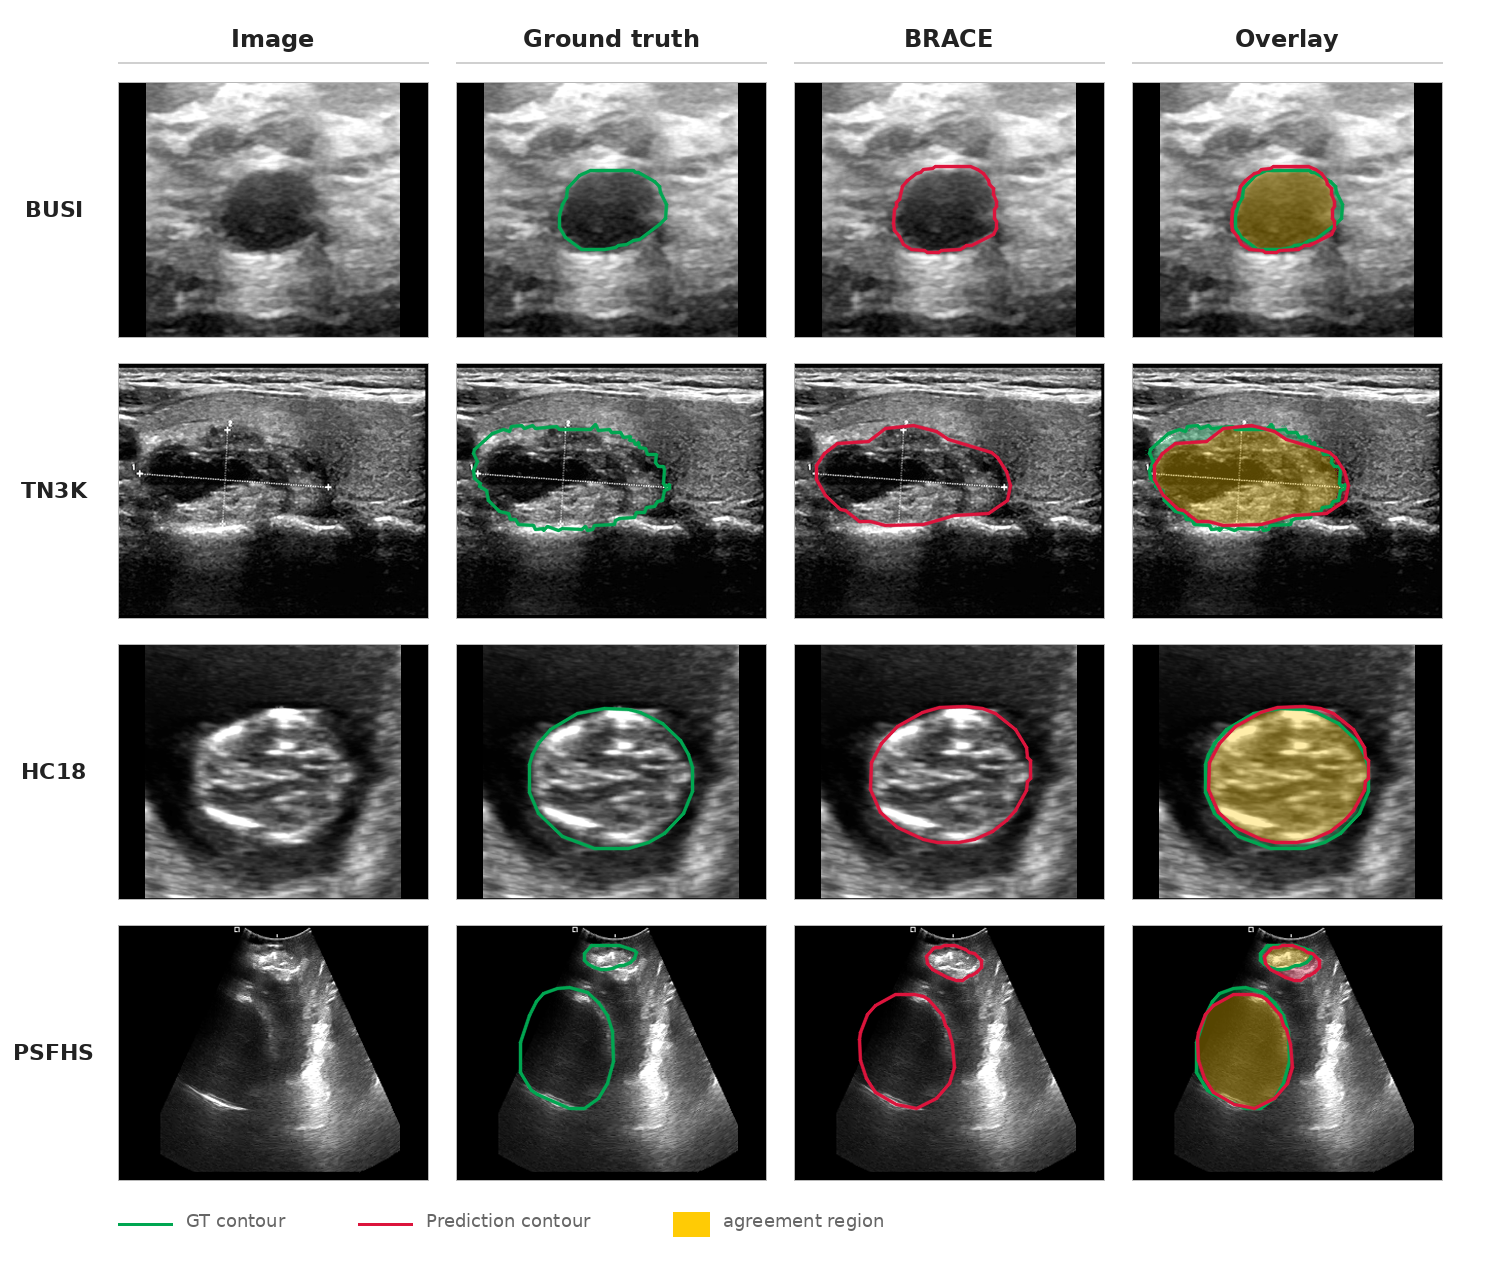
\includegraphics[width=0.86\linewidth]{compare.png}
    \caption{Qualitative BRACE segmentation examples on challenging ultrasound cases. Each row shows the input image, ground-truth boundary, BRACE prediction boundary, and an overlay view. Green contours denote ground-truth boundaries, red contours denote BRACE predictions, and yellow regions indicate agreement. The examples highlight boundary coherence and remaining structural errors in difficult cases.}
    \label{fig:compare}
\end{figure*}
\begin{table*}[!t]
\caption{HC18 segmentation performance under different labeling ratios following the BiPCC fetal-head protocol. Distance metrics use the official HC18 pixel-size metadata.}
\centering
\scriptsize
\setlength{\tabcolsep}{3pt}
\begin{tabular}{l|c|cccc|cccc}
\toprule
\multirow{2}{*}{\textbf{Method}} & \multirow{2}{*}{\textbf{Venue}} 
& \multicolumn{4}{c|}{\textbf{10\% labeled}} 
& \multicolumn{4}{c}{\textbf{20\% labeled}} \\
\cline{3-10}
& & DSC(\%)$\uparrow$ & Jaccard(\%)$\uparrow$ & 95HD(mm)$\downarrow$ & ASD(mm)$\downarrow$
  & DSC(\%)$\uparrow$ & Jaccard(\%)$\uparrow$ & 95HD(mm)$\downarrow$ & ASD(mm)$\downarrow$ \\
\hline
UA-MT~\cite{b41} & MICCAI’19 & 78.89 & 73.21 & 5.15 & 6.83 & 86.13 & 80.19 & 3.14 & 4.10 \\
S4CV~\cite{b42} & ECCV’22 & 82.76 & 77.92 & 2.15 & 3.42 & 88.07 & 81.97 & 1.58 & 3.42 \\
MC-Net~\cite{b43} & MedIA’22 & 82.90 & 78.55 & 2.15 & 3.41 & 89.02 & 83.86 & 1.44 & 2.31 \\
BCP~\cite{b44} & CVPR’23 & 81.23 & 76.17 & 3.55 & 4.63 & 87.04 & 81.45 & 2.69 & 2.91 \\
ABD~\cite{b45} & CVPR’24 & 83.07 & 78.50 & 2.09 & 3.16 & 88.89 & 83.11 & 1.44 & 2.21 \\
MiDSS~\cite{b46} & CVPR’24 & 80.73 & 75.26 & 4.43 & 5.66 & 86.79 & 80.40 & 2.76 & 3.37 \\
LeFeD~\cite{b47} & TMI’24 & 83.19 & 78.78 & 2.09 & 3.12 & 89.63 & 84.09 & 1.40 & 1.91 \\
KnowSam~\cite{b49} & TMI’25 & 81.70 & 76.84 & 2.38 & 3.76 & 87.22 & 82.89 & 2.14 & 2.64 \\
PICK~\cite{b48} & IJCV'25 & 82.04 & 78.12 & 2.24 & 3.53 & 87.31 & 82.67 & 1.58 & 2.33 \\
VerSemi~\cite{b50} & TMI’25 & 82.97 & 78.60 & 2.14 & 3.33 & 89.42 & 83.98 & 1.66 & 2.17 \\
BiPCC~\cite{b51} & 2025 & 83.32 & 79.14 & 1.94 & 2.85 
& 89.75 & 84.44 & 1.31 & 1.87 \\
BRACE (Ours) & 2025 & 96.88 & 94.64 & 1.70 & 0.60 
& 97.01 & 94.92 & 1.40 & 0.52 \\

\bottomrule
\end{tabular}
\label{tab:hc18_results}
\end{table*}
\subsubsection{Quantitative Comparison}

\noindent\textbf{PSFHS and HC18 under the BiPCC protocol.} Tables~\ref{tab:psfhs_results} and~\ref{tab:hc18_results} report DSC, Jaccard, 95HD, and ASD under the reference BiPCC-style protocol. HC18 distances use official pixel-size metadata, whereas PSFHS distances use the assumed-spacing protocol-scale convention described in Section~4.2. BRACE obtains strong HC18 performance and improves the low-label PSFHS setting, showing that boundary-reliability knowledge transfer is effective when annotations are scarce. On PSFHS, the 20\% PS component (82.32\%) remains below fetal-specific prototype methods such as BiPCC, indicating that task-specific prototype knowledge can complement generic boundary-reliability alignment for very small structures.

\textbf{BUSI and TN3K under the Shape Prior protocol.} Table~\ref{tab:final_busi_tn3k} shows DSC and IoU under 1/2, 1/4, and 1/8 labeled ratios. Under the 1/8 setting, BRACE achieves 78.52\% Dice on BUSI and 83.66\% Dice on TN3K. The results confirm that the proposed boundary-reliability design is applicable to both breast and thyroid ultrasound segmentation, while the non-monotonic low-label trends motivate broader repeated-seed studies. Representative component ablations are in Table~\ref{tab:ablation_full}.

\textbf{Summary.} Overall, the reported results support BRACE as a general knowledge-guided framework across lesion and fetal-ultrasound segmentation. The remaining PS limitation in Table~\ref{tab:psfhs_results} further motivates prototype-aware extensions for fetal-specific small structures.

\subsubsection{Qualitative Analysis}

Fig.~\ref{fig:compare} presents BRACE segmentation examples on challenging ultrasound cases across BUSI, TN3K, HC18, and PSFHS. The prediction and overlay columns show that BRACE generally preserves compact and coherent foreground structures, while residual discrepancies remain near weak or ambiguous boundaries. These visualizations support the quantitative evidence that boundary-reliability knowledge alignment reduces pseudo-label distortion and improves anatomical fidelity.

\paragraph{Knowledge-transfer verification and low-label stability.} The central hypothesis is that when pseudo-label errors are structurally correlated, boundary-reliability knowledge alignment can reduce their propagation. The reported results are consistent with this hypothesis in three ways. First, boundary-aware performance on HC18 and TN3K indicates that the learned representation preserves structural knowledge rather than only region overlap. Second, low-label PSFHS results show PS/FH improvement when labeled data are scarce, although the 20\% PS setting remains challenging. Third, the qualitative examples (Fig.~\ref{fig:compare}) show compact BRACE predictions and expose residual boundary discrepancies, consistent with boundary-knowledge alignment from FBWA and reliability-aware transfer from RCT. Failure cases (Fig.~\ref{fig:failure_cases}) occur mainly where structural cues are inherently weak, motivating prototype-aware extensions for fetal ultrasound.


\subsection{Ablation Study}

\par\smallskip
\refstepcounter{table}\label{tab:ablation_full}
\noindent\textbf{Table~\thetable}\\[0.1em]
\noindent\parbox{\linewidth}{\footnotesize Representative component ablation on BUSI and TN3K under the low-label 1/8 setting. ``Baseline'' removes FBWA, SORP, CAE, and RCT.}
\par\smallskip
\begin{center}
{\scriptsize
\setlength{\tabcolsep}{3pt}
\begin{tabular}{l|cc|cc}
\toprule
\multirow{2}{*}{\textbf{Variant}} & \multicolumn{2}{c|}{\textbf{BUSI 1/8}} & \multicolumn{2}{c}{\textbf{TN3K 1/8}} \\
\cline{2-5}
& Dice & IoU & Dice & IoU \\
\midrule
Baseline & 75.37 & 66.58 & 79.50 & 70.31 \\
BRACE & \textbf{77.69} & \textbf{69.12} & 81.02 & 72.04 \\
w/o FBWA & 75.19 & 65.53 & 78.89 & 69.72 \\
w/o SORP & 76.35 & 66.61 & \textbf{81.96} & \textbf{73.17} \\
w/o RCT & 76.57 & 67.41 & 81.00 & 72.32 \\
w/o CAE & 75.39 & 65.49 & 80.88 & 71.80 \\
\bottomrule
\end{tabular}
}
\end{center}
\par\smallskip

Table~\ref{tab:ablation_full} reports the main structural components on BUSI and TN3K. The full configuration improves over the stripped baseline on both datasets, supporting the benefit of reliability-calibrated boundary knowledge transfer. The component effects are not strictly monotonic on every dataset: on TN3K, removing SORP slightly increases the region score in this run. This behavior indicates that FBWA, SORP, RCT, and CAE interact with dataset texture, pseudo-label reliability, and auxiliary-decoder stability rather than acting as independent additive terms.

\par\smallskip
\begin{center}
  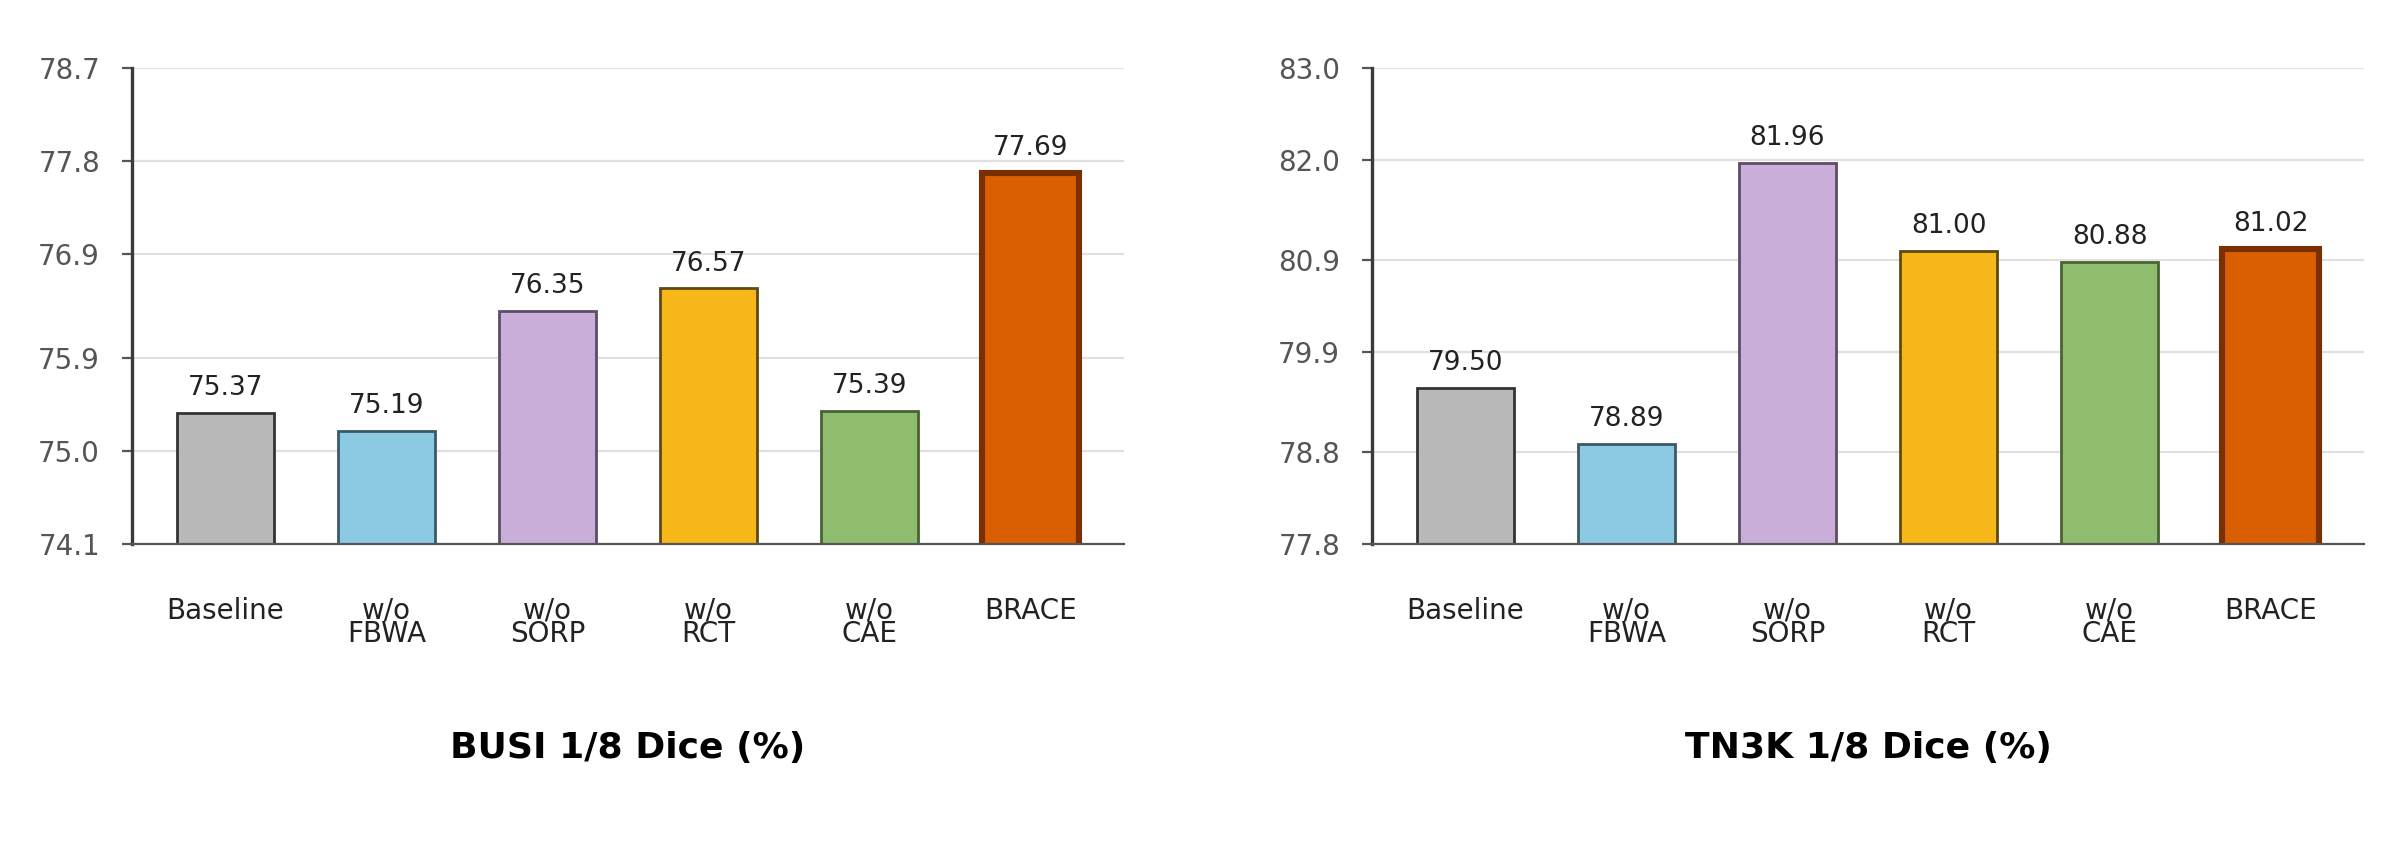
\includegraphics[width=\linewidth]{component_effect_summary.png}
\end{center}
\captionof{figure}{Component-effect visualization on BUSI and TN3K under the 1/8 labeled setting. Values are derived from Table~\ref{tab:ablation_full}. The plot summarizes component interactions and indicates that module effects depend on dataset texture and auxiliary-decoder stability.}
\label{fig:component_effect}
\par\smallskip

\par\smallskip
\refstepcounter{table}\label{tab:psfhs_component_analysis}
\noindent\textbf{Table~\thetable}\\[0.1em]
\noindent\parbox{\linewidth}{\footnotesize PSFHS component analysis. Values are PS/FH Dice (\%). The analysis inspects module interactions on the small PS structure; the main comparison results are reported in Table~\ref{tab:psfhs_results}.}
\par\smallskip
\begin{center}
{\scriptsize
\setlength{\tabcolsep}{3pt}
\resizebox{\linewidth}{!}{%
\begin{tabular}{l|cc}
\toprule
\textbf{Variant} & \textbf{10\% labeled} & \textbf{20\% labeled} \\
\midrule
Baseline & 57.10 / 80.49 & 71.26 / 89.59 \\
BRACE (class-aware weighted Dice) & 70.85 / 90.32 & 73.40 / 92.24 \\
w/o FBWA & 72.61 / 91.49 & 62.55 / 91.72 \\
w/o SORP & \textbf{78.77} / 90.27 & 75.37 / 91.21 \\
w/o RCT & 74.82 / \textbf{91.91} & 72.97 / 90.92 \\
w/o CAE & 71.50 / 90.86 & 66.88 / 89.55 \\
BRACE (merged foreground objective) & 72.14 / 89.91 & \textbf{76.80} / \textbf{92.26} \\
\bottomrule
\end{tabular}
}%
}
\end{center}
\par\medskip

The PSFHS component analysis in Table~\ref{tab:psfhs_component_analysis} highlights the difficulty of the PS component. PS is much smaller and more variable than FH, and module interactions are stronger than on single-foreground lesion datasets. SORP and RCT provide clear gains under the 10\% setting, while the merged-foreground objective improves the 20\% PS/FH Dice in this analysis. The main comparison follows the class-aware PS/FH training path, and the merged-foreground result is included to show how objective design affects small-structure stability. This result is consistent with our limitation analysis: BRACE is a general boundary-reliability knowledge alignment framework, while fetal-specific prototype knowledge remains promising for further improving PS.

\subsection{Sensitivity Analysis}

\begin{table*}[!t]
\centering
\scriptsize
\setlength{\tabcolsep}{2pt}
\renewcommand{\arraystretch}{1.06}
\caption{PSFHS sensitivity analysis for $\lambda_{\mathrm{adv}}$, the SORP coupling coefficient, and $\delta$ under 10\% labeled data. Values are reported as paired PS/FH metrics with the corresponding dispersion from the experiment summaries; distance values use the assumed-spacing protocol-scale convention.}
\label{tab:psfhs_sensitivity}
\resizebox{\textwidth}{!}{%
\begin{tabular}{ccccccc}
\hline
\multirow{2}{*}{$\lambda_{\mathrm{adv}}$} & 
\multirow{2}{*}{$\lambda_{\mathrm{SORP}}$} & 
\multirow{2}{*}{$\delta$} &
\multicolumn{4}{c}{Metrics $\uparrow$ (higher is better) / $\downarrow$ (lower is better)} \\
\cline{4-7}
 & & & Dice (\%) $\uparrow$ & Jaccard (\%) $\uparrow$ & HD95$^\dagger$ $\downarrow$ & ASD$^\dagger$ $\downarrow$ \\
\hline
0.05 & 0.2 & 0.1 & 78.91 / 84.72 $\pm$ 1.25 & 73.12 / 81.65 $\pm$ 1.31 & 5.03 / 4.58 $\pm$ 1.71 & 2.74 / 1.82 $\pm$ 0.22 \\
0.10 & 0.2 & 0.1 & \textbf{79.39 / 85.23} $\pm$ \textbf{1.06} & \textbf{74.11 / 82.67} $\pm$ \textbf{1.14} & \textbf{4.78 / 4.17} $\pm$ \textbf{1.63} & \textbf{2.59 / 1.56} $\pm$ \textbf{0.18} \\
0.15 & 0.2 & 0.1 & 78.74 / 84.63 $\pm$ 1.18 & 73.45 / 82.04 $\pm$ 1.22 & 4.96 / 4.36 $\pm$ 1.68 & 2.63 / 1.62 $\pm$ 0.19 \\
0.10 & 0.3 & 0.1 & 78.88 / 84.57 $\pm$ 1.15 & 73.26 / 81.91 $\pm$ 1.21 & 4.89 / 4.31 $\pm$ 1.67 & 2.67 / 1.60 $\pm$ 0.20 \\
0.10 & 0.2 & 0.2 & 78.65 / 84.28 $\pm$ 1.22 & 73.01 / 81.53 $\pm$ 1.27 & 5.11 / 4.52 $\pm$ 1.74 & 2.72 / 1.69 $\pm$ 0.21 \\
\hline
\end{tabular}
}
\end{table*}
\begin{table}[!h]
\caption{Sensitivity analysis of $\lambda_{\text{adv}}$ and the SORP coupling coefficient on BUSI (1/8).}
\centering
\scriptsize
\begin{tabular}{c|cc|c|cc}
\toprule
\multicolumn{3}{c|}{\textbf{Varying} $\lambda_{\text{adv}}$ (fix $\lambda_{\text{SORP}}=0.2$)} & \multicolumn{3}{c}{\textbf{Varying} $\lambda_{\text{SORP}}$ (fix $\lambda_{\text{adv}}=0.1$)} \\
\midrule
$\lambda_{\text{adv}}$ & Dice (\%) & IoU (\%) & $\lambda_{\text{SORP}}$ & Dice (\%) & IoU (\%) \\
\midrule
0.00 & 75.71 & 67.47 & 0.00 & 75.71 & 67.47 \\
0.05 & 76.52 & 68.21 & 0.10 & 76.98 & 68.63 \\
\textbf{0.10} & \textbf{77.58} & \textbf{69.11} & \textbf{0.20} & \textbf{77.58} & \textbf{69.11} \\
0.15 & 77.42 & 68.93 & 0.30 & 77.36 & 68.70 \\
0.20 & 77.10 & 68.61 & 0.40 & 77.02 & 68.33 \\
\bottomrule
\end{tabular}
\label{tab:sensitivity_analysis}
\end{table}


We analyze key structural hyperparameters to inspect whether the method is driven by a single brittle setting. Table~\ref{tab:sensitivity_analysis} reports BUSI 1/8 results when varying the FBWA generator-side weight $\lambda_{\text{adv}}$ and the SORP coupling coefficient, while Table~\ref{tab:psfhs_sensitivity} provides a PSFHS sensitivity analysis including the perturbation strength $\delta$. In the current implementation, SORP supplies an auxiliary view coupled through RCT rather than an independent standalone SORP loss; therefore, $\lambda_{\text{SORP}}$ is interpreted as a coupling coefficient in these runs.

As shown in Table~\ref{tab:sensitivity_analysis}, performance remains in a narrow range for moderate values of $\lambda_{\text{adv}}$ and the SORP coupling coefficient, indicating that the structural feedback does not require aggressive tuning in these reported runs. The current implementation uses a conservative FBWA weight and treats SORP primarily as an auxiliary view coupled through RCT, rather than as an always-beneficial standalone loss. This interpretation is consistent with the ablation in Table~\ref{tab:ablation_full}, where SORP helps some settings but is not strictly monotonic on TN3K.

For PSFHS, Table~\ref{tab:psfhs_sensitivity} shows that moderate changes around the default setting lead to limited variation in the paired PS/FH metrics. The small PS component remains sensitive to class imbalance and fetal-specific anatomy; therefore, objective design and prototype-aware reliability calibration remain important directions for improving PS stability.


\subsection{Model Complexity and Efficiency}

We further analyze the computational cost of our framework as an implementation-level estimate. With a ResNet-34 backbone and U-Net-style decoder, the baseline network contains about 24.0M parameters and 32.2 GFLOPs per $512\times512$ input (see Table~\ref{tab:flops}). Adding FBWA and SORP increases the training-graph complexity to 25.6M parameters and 33.5 GFLOPs, corresponding to a 6.7\% parameter and 4.0\% FLOP increase. The full BRACE configuration, including CAE, contains 26.1M parameters and 33.8 GFLOPs, corresponding to an 8.8\% parameter and 5.0\% FLOP increase over the baseline. These numbers use a $512\times512$ reference input, whereas the reported segmentation experiments resize images to $320\times320$ and train with $256\times256$ crops. Params/FLOPs include modules active during training, while the final segmentation inference path uses the segmentation network without the FBWA critic. The measured wall-clock summary indicates that, for a 200-epoch BUSI run with batch size 16, the baseline and BRACE require approximately 2.8 h and 3.1 h, respectively, giving a 10.7\% wall-clock overhead.
\begin{table}[!t]
\caption{Implementation-level complexity estimate on a $512\times512$ reference input. Params/FLOPs include modules active during training, while inference time is measured for the segmentation forward path.}
\centering
\scriptsize
\begin{tabular}{lccc}
\toprule
\textbf{Model} & \textbf{Params} & \textbf{FLOPs} & \textbf{Infer. time} \\
& \textbf{(M)} & \textbf{(G)} & \textbf{(ms)} \\
\midrule
Baseline & 24.0 & 32.2 & 22.2 \\
+ FBWA & 25.5 & 33.4 & 22.8 \\
+ FBWA + SORP & 25.6 & 33.5 & 23.1 \\
+ FBWA + SORP + CAE & \textbf{26.1} & \textbf{33.8} & \textbf{23.3} \\
\bottomrule
\end{tabular}
\label{tab:flops}
\end{table}
\begin{figure*}[!t]
    \centering
    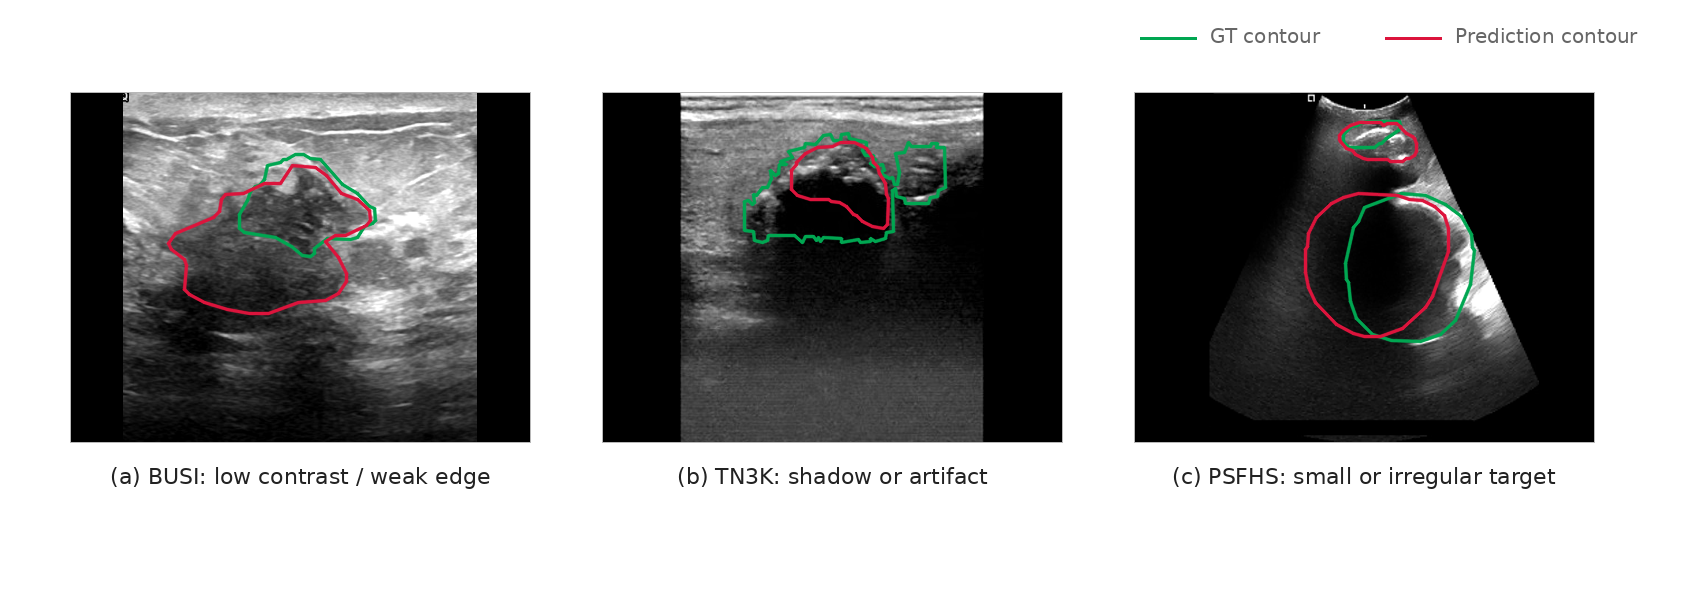
\includegraphics[width=0.92\linewidth]{failure_cases.png}
    \caption{Failure and limitation cases from BUSI, TN3K, and PSFHS. Green contours denote ground-truth boundaries and red contours denote BRACE predictions. The examples illustrate typical remaining errors under weak contrast, acoustic shadowing or artifacts, and small or irregular fetal targets.}
    \label{fig:failure_cases}
\end{figure*}
\subsection{Limitations and Future Work}

Despite its promise, BRACE has several limitations and protocol-scope considerations. First, the main experiments intentionally follow the public Shape Prior and BiPCC reference protocols to maintain comparability with prior semi-supervised ultrasound studies. Some protocol files define image-level benchmark partitions with a single evaluation set rather than a separate validation/test hierarchy; future studies with patient or video identifiers could further strengthen patient-level generalization analysis. Second, the main tables are based on a single recorded seed and a fixed configuration including strong augmentation, applicable copy-paste augmentation, adaptive class-aware weighted Dice, test-time augmentation, and recorded post-processing settings. Multi-seed runs and a fuller factorial ablation would provide a stronger statistical and attribution analysis. Third, PSFHS distance metrics use an assumed 0.4 mm/pixel native spacing because the available MHA headers contain placeholder spacing; pixel-distance reporting or verified spacing metadata would make cross-study calibration clearer. Fourth, HD95/ASD are undefined when only one of prediction or ground truth is empty, and our aggregate means exclude those NaN entries. Reporting valid-sample counts and failure counts would further clarify distance-metric robustness, especially for small PS structures. Finally, as shown in Fig.~\ref{fig:failure_cases}(a)--(c), the model occasionally fails in extremely challenging cases, including low-contrast lesions, heavy speckle interference, or highly irregular and ambiguous boundaries. Future work will therefore prioritize multi-seed statistics, patient-level validation where identifiers are available, explicit distance calibration, failure-count reporting, and prototype-aware reliability calibration.

We also plan to develop lightweight architectural variants through neural architecture search or knowledge distillation techniques, enabling efficient inference while preserving boundary-reliability knowledge for mobile and embedded ultrasound analysis systems. Finally, the current framework relies on handcrafted structural operators (e.g., Sobel filters) to extract boundary cues. While effective, these may not optimally generalize across diverse ultrasound domains or imaging protocols. We will investigate learnable boundary-knowledge extraction modules that can adaptively learn domain-specific edge representations through end-to-end training, potentially replacing fixed operators with trainable convolutional layers or attention mechanisms that better capture anatomical boundary characteristics across different ultrasound modalities.




\section{Conclusion}

Our findings suggest that semi-supervised ultrasound segmentation should not transfer pseudo-labels as isolated pixel targets. When errors are structurally correlated rather than pixel-wise independent, standard consistency objectives may propagate boundary drift. BRACE addresses this issue by formulating SSL as boundary-reliability knowledge alignment and by coupling feature-boundary Wasserstein alignment (FBWA), structure-oriented residual perturbation (SORP), and reliability-calibrated co-teaching (RCT).

Experiments on four public datasets (BUSI, TN3K, PSFHS, HC18) demonstrate that BRACE can provide competitive region accuracy and boundary-aware behavior under limited annotations. Ablations and qualitative results support the plausibility of structural boundary knowledge, perturbation-based auxiliary knowledge, and reliability-aware pseudo-label transfer under the Shape Prior and BiPCC evaluation protocols. The framework offers a practical knowledge-based direction for reliable semi-supervised ultrasound segmentation, while future work will broaden multi-seed evidence and explore prototype-aware knowledge calibration for small fetal structures and lightweight variants for deployment.

\section{Data Availability Statement}

The datasets used in this study are publicly available from the original BUSI~\cite{b1}, TN3K~\cite{b4}, PSFHS~\cite{b53}, and HC18~\cite{b54} releases. No new clinical dataset was collected for this work. The implementation and scripts for reproducing the reported experiments are available at \url{https://github.com/YanHu826/addressing_boundary_ambiguity}. The released artifacts include split hashes, run manifests, and per-case metric files where available. For PSFHS, the reproducibility artifacts follow the BiPCC-aligned 4,000-image image-level partition; patient/video identifiers are not included in the available protocol files.

\section{Ethics Statement}

This research does not require additional ethics approval from our institution's ethics committee as it uses only publicly available datasets that have been previously published and are openly accessible for research purposes. All datasets used in this study—BUSI~\cite{b1}, TN3K~\cite{b4}, PSFHS~\cite{b53}, and HC18~\cite{b54}—were collected and released by their respective institutions with appropriate ethical approvals and informed consent procedures completed prior to public release. The dates and reference numbers of the ethical approvals obtained for each dataset are documented in the original publications cited in this manuscript~\cite{b1,b4,b53,b54}.

\section{Funding}

This research did not receive any specific grant from funding agencies in the public, commercial, or not-for-profit sectors.

\section{Declaration of Generative AI and AI-Assisted Technologies in the Manuscript Preparation Process}

During the preparation of this work, the authors used AI-assisted language editing tools to support language polishing, consistency checking, and LaTeX formatting. After using these tools, the authors reviewed and edited the content as needed and take full responsibility for the content of the article.

\section{Declaration of Competing Interest}

The authors declare that they have no known competing financial interests or personal relationships that could have appeared to influence the work reported in this paper.

\printcredits

%% Loading bibliography style file
%\bibliographystyle{model1-num-names}
\bibliographystyle{cas-model2-names}

% Loading bibliography database
\bibliography{cas-refs}

\end{document}
